\documentclass[12pt]{report}
\usepackage{setspace}
%\usepackage{subfigure}

\pagestyle{plain}
\usepackage{amssymb,graphicx,color}
\usepackage{amsfonts}
\usepackage{latexsym}
\usepackage{amsmath}
\usepackage{algorithm}
\usepackage{algorithmicx}
\usepackage{algpseudocode}

\newtheorem{theorem}{THEOREM}
\newtheorem{lemma}[theorem]{LEMMA}
\newtheorem{corollary}[theorem]{COROLLARY}
\newtheorem{proposition}[theorem]{PROPOSITION}
\newtheorem{remark}[theorem]{REMARK}
\newtheorem{definition}[theorem]{DEFINITION}
\newtheorem{fact}[theorem]{FACT}

\newtheorem{problem}[theorem]{PROBLEM}
\newtheorem{exercise}[theorem]{EXERCISE}
\def \set#1{\{#1\} }

\newenvironment{proof}{
PROOF:
\begin{quotation}}{
$\Box$ \end{quotation}}


\graphicspath{
  {/home/hege/Documents/Thesis/msc-thesis/}
  {/home/hege/Documents/Thesis/msc-thesis/figures/}
}

\newcommand{\nats}{\mbox{\( \mathbb N \)}}
\newcommand{\rat}{\mbox{\(\mathbb Q\)}}
\newcommand{\rats}{\mbox{\(\mathbb Q\)}}
\newcommand{\reals}{\mbox{\(\mathbb R\)}}
\newcommand{\ints}{\mbox{\(\mathbb Z\)}}

%%%%%%%%%%%%%%%%%%%%%%%%%%


\title{  	{ 
\includegraphics[scale=.5]{ucl_logo.png}}\\
{{\Huge Deep Hyperbolic Semantic Embedding Model for Zero-Shot Learning}}\\
%{\large }\\
		}
\date{Submission date: Day Month Year}
\author{Hermanni H{\"a}lv{\"a} \thanks{
{\bf Disclaimer:}
This report is submitted as part requirement for the MSc CSML degree at UCL. It is
substantially the result of my own work except where explicitly indicated in the text.
The report may be freely copied and distributed provided the source is explicitly acknowledged
\newline  %% \\ screws it up
}
\\ \\
MSc. Computational Statistics and Machine Learning\\ \\
Supervisor: Prof. Bradley Love}

\begin{document}
 
\onehalfspacing
\maketitle

\begin{abstract}
  Even though \textit{deep learning} models have achieved state-of-the-art results on virtually all image classification tasks, their ability to generalize into novel environments remains constrained. One of the most challenging problems which illustrates this is \textit{zero-shot learning}. In this task the training and test sets are completely disjoint; that is, at test time the model tries to label images from object classes that it has never seen before. A common approach to this problem has been to learn a mapping from training images to a semantic embedding space that contains all the class labels. Zero-shot classification is done by mapping previously unseen classes of images into the embedding space where nearest neighbour search is performed. A limitation of the embeddings spaces employed by previous works is that they only capture semantic similarity of labels, but fail to account for more complex hierarchical semantic relations that could further improve generalization performance. For instance, research has shown that humans perform classification by traversing a hierarchy of semantic categories and associated taxonomy of visual memories. Thus even if we are shown a picture of an uknown dog breed, we can still say that it belong to the higher level categories 'dogs', 'mammals' and so forth. 

This thesis aims is to endow deep learning with similar type of rich hierarchical semantic understanding and investigate its benefits on zero-shot learning. To do this, we utilize the recent idea of hyperbolic embeddings, which have been shown to outperform Euclidean ones at representing hierarchical graphs. In particular, we introduce a \textit{Deep Hyperbolic Semantic Embedding model} which use a deep learning model to map into a hyperbolic semantic embedding space. The model was evaluated on  \dots and the results show that \dots to our knowledge this thesis is the first work to show \dots

\end{abstract}

\chapter*{Acknowledgements}
\thispagestyle{empty}
First, I would like to thank my supervisor Prof. Bradley Love, for all of his guidance, support and loads of great ideas. His genuine interest in the project and desire to help out really made the entire process very enjoyable. Massive thanks also to Olivia Guest, and Sebastian Bobadilla-Suarez for sharing their ideas and for pointing me to loads of relevant research I likely would have otherwise missed. Thank you to Adam Hornsby for helping me get my head around the different word embedding methods and for how I should think about presenting the project. Special thank you to Brett Roads for being incredibly helpful with setting up and helping to maintain the compute resources and data, which were required for this project; I was so impressed with the whole set up and how well it all functioned. For sure, nothing would have come of this project had I not received all this help, so for that - thank you!

\clearpage

\tableofcontents
\listoffigures
\listoftables
\setcounter{page}{1}

\chapter{Notes}
\begin{itemize}
    \item Do I clearly state that CNNs are the state-of-the-art on image classification, give some example of current results / super human performance or when they wont competitions first time
    \item we have created Deep-Glove because a.) it has lower dimensionality of w2v vector b.) newever DNN to make the model comparable to ours.
\end{itemize}

\chapter[Introduction]{Introduction\raisebox{.3\baselineskip}{\normalsize\footnotemark}}
\footnotetext{All the code developed for this project can be accessed at https://github.com/HHalva/msc-thesis}

\section{Project Motivation}
Over the past decade deep learning has achieved state-of-the-art results on virtually all computer vision tasks \cite{Goodfellow2016}. The impressive performance of these models has, in turn, propelled paramount improvements in a wide range of application areas such as autonomous vehicles\cite{Bojarski2016}, face recognition \cite{Taigman2014} and robotics \cite{Finn2015}\cite{Ganegedara2017}. Despite the many successes of deep learning, most of the achievements rely on well defined training and test envionments; the generalization performance of these models is still far from that of the human visual system. One particularly challenging task that illustrates this is zero-shot learning, that is, making predictions about previously unseen classes of images. The aim of this thesis is to improve the generalization performance of deep learning models in the context of zero-shot learning. We approach this by attempting to teach the models a more human-like hierarchical understanding of object categorization.

Some of the biggest advances in deep learning have come in the area of image classification. Inspired by the breakthrough performance of Krizhevsky \textit{et al.} \cite{Krizhevsky2012} on the ImageNet 2012 classification challenge \cite{JiaDeng2009}, researchers have produced increasingly sophisticated deep learning architectures and as a result have recently surpassed human performance on this task \cite{Dodge2017}. Yet, the classifications these models are able to perform are inherently restricted; any new image can only be labelled as one of the training classes. In other words, it is not possible to make correct predictons about any new classes of images without further training data on them. Zero-shot learning \cite{Palatucci2009} tries to address this limitation.

\begin{figure}
  \centering
	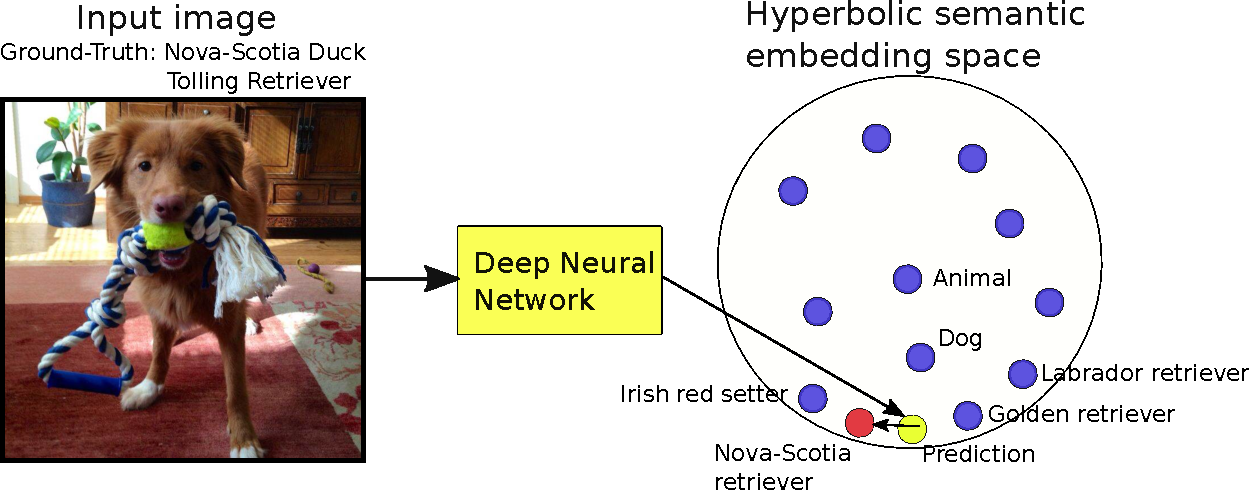
\includegraphics[width=\textwidth]{introzsl}
	\caption{Hypothetical example of zero-shot classfication. Assume that we have used training images and their embedding vectors (blue dots) to learn a mapping from image features into the hyperbolic embedding space. Next an image from a previously unseen class is encountered, since the entity in the image looks a bit like a mix of golden retriever and Irish red setter, the predicted semantic embedding falls in between those two, which indeed happens to be close to the ground-truth embedding: Nova-scotia Duck Tolling Retriever.}
	\label{fig:intro}
\end{figure}

Whilst making predictions about previously unseen objects may sound impossible at first, humans can easily do this, under certain conditions. To see this, imagine for a moment that you have never seen a Zebra, but your zoologist friend aptly tells you that ``a Zebra is like a horse with black and white stripes''. The next time you see an animal that fits this description, you could recognize the Zebra, even though you have never seen one before! This represents the power of auxillary semantic information in image classification. In typical zero-shot recognition models this information comes in the form of word embeddings. These are usually constructed so that words which occur in a similar semantic context are placed close to each other in a vector space. The classic zero-shot approach is to learn a mapping from training images into the word embedding. This mapping is then used to project any novel images into the embedding space where they can be classified using nearest neighbour search (see Figure \ref{fig:intro} for an example). 

A fundamental assumption that underpins this approach is that there is a close relationship between contextual semantic similarity and visual similarity. While this is often true \cite{Deselaers2011}, these similarity-based embeddings fail to account for more complex, hierarchical, semantic relations, which could better reflect visual characteristics of objects. For instance, biological organisms can be organised in a hierarchical taxonomy based on their physical traits \cite{Ohl2015}. In fact, the rich visual understanding that humans display is based on semantic and visual hierarchy of objects \cite{Joliceur1984}. A related limitation is that similarity-based embeddings don't easily accomodate for subordinate relations: it might be possible to reason that the words 'cat' and 'pet' are groupped near each other but cannot deduce whether 'pet' is a 'cat' or 'cat' a 'pet'. In contrast to this, a human who sees a cat of an uknown breed, can traverse up the hierarchy and group it under the higher level category of cat, or even animals and mammals if necessary. 

We propose a deep learning model with the ability to reason in semantic hierarchies by training the model to project input images into a hyperbolic embedding space. Hyperbolic geometry has recently been shown to be well suited for capturing hierarchical graph structures such as semantic taxonomies \cite{Nickel2017, Chamberlain2017}. We hypothesize that the resulting structure of the embedding space will better reflect the visual similarities of different objects, which should improve zero-shot classification. Our central research question can thus be stated as: 
\begin{itemize}
  \item \textit{Does semantic hierarchical knowledge in the form of hyperbolic embeddings help improve the zero-shot prediction capability of deep learning models?}
\end{itemize}

Our research into zero-shot learning is also motivated by the fundamental scarcity of readily available labelled data. This is a problem for many real-world applications of deep learning. As an example, for autonomous vehicles to operate safely, they need to be able to perform inference in novel visual scenarios. Being able to identify an uknown object as a living entity can be incredibly valueable, even if more precise classification is not possible.

Overall our resuls\dots\dots\dots

In the remainder of this chapter we provide a brief overview of our methodology and how it fits in the existing literature on zero-shot learning. We also summarize our key results more explicitly and the main take-aways for future research. In Chapter \ref{ch:backg} we cover the necessary technical background for this project and review literature in more detail. Chapter \ref{} presents our approach in detail, and the full results from our experiments are given in Chapter \ref{}. Chapter \ref{} concludes our work with a discussion of the results and presents ideas for future research.

\section{Summary of Key Literature}
Modern deep neural networks take the form of Convolutional Neural Networks \cite{Lecun2015}, which learn a hierarchical visual representation of objects over multiple layers of convolution operations. Typically these models are trained against one-hot-encoded vectors of class labels: if there are N classes, the label of each image will be N-dimensional vector with a $1$ in the dimension of the correct class and 0s in all other dimensions. Crucially, these vectors are orthogonal to each other. This is why standard deep learning models do not learn to capture any semantic relations between the visual objects, eventhough the hierarchical visual features that the model learn would be well suited for this. As a consequence, a standard deep learning model is not able to communicate, for example, that cats and dogs are both mammals if training labels are available only for the former two. Those few works that have attempted to use multi-level lables \cite{Wang2015}, \cite{Peterson2018}, have only used up to three levels of hierarchy. Whilst their results are promising, such shallow hierarchies are unable to represent the full complexity of semantic relations. Additionally, the generalization ability of these models has only been tested on training labels but not on zero-shot prediction.

As discussed above, zero-shot learning has instead focused on improving generalization performance via word embeddings \cite{Palatucci2009, Socher, Huang2012, Frome2013, Norouzi2013}. Note that this is possible because the embedding spaces are created so that they contain all the possible labels, including zero-shot ones. Hence, projecting images into this space can help with classification. Several methods have been used to create such all encompassing label-vector spaces. The most popular has been to utilize the word2vec family of models \cite{Mikolov, Mikolov2013}. These take in a large corpus of text, such the 5.2 billions words long Wikipedia data, and place words that occur in a similar context near to each other in the resulting, Euclidean, embedding space. For example, the model that is most similar to ours, DeViSE \cite{Frome2013}, uses a deep neural network to map into this space. 

As alluded to earlier, similarity embeddings fail to capture the semantic hierarchy of objects, which is how humans categorize the world around us \cite{Rosch1976, Joliceur1984}. One likely reason why hierarchical relations haven't been used by previous works is that embedding them in Euclidean space is difficult. Only very recently have Nickel and Kiela \cite{Nickel2017} and Chamberlain \textit{et al.} \cite{Chamberlain2017} shown that this can be done much more easily in hyperbolic geometry, and thus have introduced the idea of hyperbolic graph embeddings.

The main property than distinguishes hyperbolic spaces from Euclidean ones is that they have a constant negative curvature \cite{Greenberg1994}. The consequence of this is that the area of a hyperbolic sub-space, such as a circle, expands exponentially as we move away from the centre, as opposed to the quadratic growth in Euclidean geometry. This exponential growth is also the rate at which hierarchical trees, with a constant branching factor, grow; hence the suitability of hyperbolic spaces to embed semantic hierarchies \cite{Nickel2017, Chamberlain2017}.

\section{Summary of Our Approach}
We started by constructing a hyperbolic embedding that contains all the possible ground truth labels. For this we used the Poincare embedding model of Nickel and Kiela \cite{Nickel2017}. More specifically, this model was applied to the WordNet lexical data base which consists of 82,000 nouns and their semantic relations in the form of a hierarchical graph. As a result, we acquired 10-dimensional embedding vectors for all training and zero-shot labels.

In order to learn a mapping from input images into the hyperbolic space, we trained two different deep learning models on the 1000 classes of the ImageNet 2012 database \cite{JiaDeng2009}, approximately 1.3 million images. Our first model, called Deep Hyperbolic Semantic Embedding model (Deep-HSEM) employes a standard convolutional neural network in a similar vein as the DeViSE model of Frome \textit{et al.} \cite{Frome2013}. The general architecture of this model is depicted in Figure \ref{fig:dhsemIntro}. Our second one model, called Convex Hyperbolic Semantic Embedding model (Convex-HSEM) follows the approach of Norouzi \textit{et al.} \cite{Norouzi2013} and computes the predicted embeddings for zero-shot classes as convex combinations of known classes' embeddings. See Figure \ref{fig:chsemIntro} for an illustration.

\begin{figure}
  \centering
	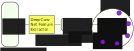
\includegraphics[width=\textwidth]{dhsemIntro}
	\caption{Illustration of the Deep-HSEM model. A standard deep learning model is ammended so that it outputs a 4096 long feature vector, which is passed through fully connected classifier layer that maps into the 10 dimensional hyperbolic space. The model parameters are learned by training images against their label embedding vectors. For zero-shot images, classification is done by nearest neighbour search in the embedding space.}
	\label{fig:dhsemIntro}
\end{figure}

\begin{figure}
  \centering
	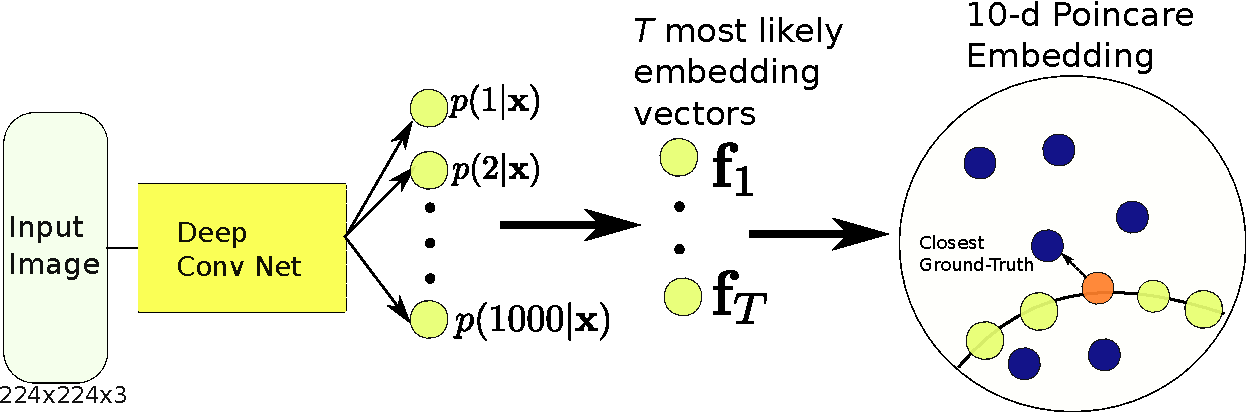
\includegraphics[width=\textwidth]{chsemIntro}
	\caption{Illustration of the Convex-HSEM model. In the first stage the model gives class predictions for any input image in terms of the 1000 training classes. Next the $T$-most likely classes and their corresponding ground-truth embedding vectors are taken. Their convex combination is then calculated in the hyperbolic space (orange dot) and nearest neighbor classification is performed subsequently. Note that a pre-trained deep learning model can be used; no traning against embedding vectors is done}
	\label{fig:chsemIntro}
\end{figure}

\section{Summary of Results}

After training, the Deep-HSEM and Convex-HSEM models were evaluated on 21,000 previously unseen zero-shot classes, obtained from the full ImageNet 2011 release \cite{JiaDeng2009}. This data set contains a total of around 13 million images. Overall, our results

\newpage

\chapter{Background} \label{ch:backg}

\section{Artificial Neural Networks \\ \& Deep Learning}
Even though deep learning is often viewed as a new technique, in reality the recent breakthroughs are underpinned by decades of related research. For instance, earliest artificial neural networks, such as Rosenblatt's Perceptron \cite{Rosenblatt1958} from the 1950s, are closely related to linear regressions; these models are all of the form $f(\mathbf{x}, \mathbf{w})=\mathbf{x}^{\intercal} \mathbf{w}$ where $\mathbf{x}$ is a vector describing some input covariate and $\mathbf{w}$ model weights. Much like in linear regression, the aim is to learn a mapping $f(\mathbf{w}, \mathbf{x}) = y$ that defines the relationship between the input $\mathbf{x}$ and some category $y$. In a simple problem, $y$ is binary and the weights $\mathbf{w}$ are learned such that the resulting hyperplane can linearly separate the data into the two. These early models were largely restricted by their assuming linear separability and there was also no computationally feasible way of training the models at the time \cite{Goodfellow2016}, \cite{JurgenSchmidhuber2015}. Nevertheless, they form the basis for nearly all Artificial Neural Networks (ANNs). 

Several steps were taken to increase to complexity of these models and to allow for non-linearities, many of them initially inspired to some degree by biological neurons \cite{Goodfellow16}. For instance, real neurons typically only fire once action potential exceeds a specific threshold \cite{Hodgkin1990}. In ANNs, similar behaviour is attained via activation functions on top of neuron outputs, most typically in the form of Rectified Linear Units (ReLU), which apply the following non-linearity: $f(\mathbf{x}, \mathbf{w})=max\{0, \mathbf{x}^{\intercal} \mathbf{w}\}$. ReLUs also improve the representational capacity of a network by imposing sparsity which can make it easier to disentangle the data \cite{Glorot2011} and hence lead to faster convergence of training \cite{Krizhevsky2012}.

Another insight borrowed from neuroscience is that intelligence stems from groups of neurons acting together rather than from individual neurons \cite{Goodfellow2016}; this idea is behind deep ANNs where several layers of neurons are connected to each other and numerous neurons are present in each layer. Below equations and Figure \ref{fig:mlp} give a simplified example of an ANN with two hidden layers:

\begin{align} \label{mlp_eq}
  \mathbf{H_1} &= max\{0, \mathbf{W}\mathbf{X} + \mathbf{B}\} \\
  \mathbf{H_2} &= max\{0, \mathbf{V}\mathbf{H_1} + \mathbf{C}\} \\ 
  \mathbf{F} &= \mathbf{Z} \mathbf{H_{2}} + \mathbf{D} 
\end{align}

\begin{figure}
  \centering
	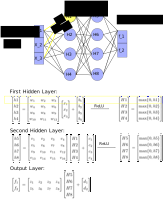
\includegraphics[width=0.8\textwidth]{mlp}
	\caption{A simple Feed-forward ANN with two hidden layers. This figure illustrates a graphical model for Equation \ref{mlp_eq} - 3.3 and explicitly shows the matrix operations performed by the different neurons on a single vector input. The output dimension is set arbitraily to be a $2\times1$ vector, which could for instance be used as class scores in binary classification; in practice, the dimension will be problem dependent.}
	\label{fig:mlp}
\end{figure}

where $\mathbf{X}$ is an $D\times N$ input data matrix of $N$ observations in the columns and $D$ is the dimension of a single observation. This matrix representation allows several datapoints to be fed through the network simultaneously, which is what is done in practice. $\mathbf{W}$, $\mathbf{V}$ and $\mathbf{Z}$ are the weights matrices of the two hidden layers and output layer respectively. The number of rows in each of the weight matrices is the number of neurons in that layer, whilst the number of columns corresponds to the input dimension. Notice also that constant bias matrices $\mathbf{B}$, $\mathbf{C}$, and $\mathbf{D}$ are added to the neuron outputs. These bias matrices are akin to intercepts in regression analysis and increase the representation ability of the model. Mathematically these matrix operations are just affine transformations on the input followed by ReLUs, which are applied elementwise. The output of each layer is thus a matrix, here $\mathbf{H_1}$ and $\mathbf{H_2}$, where each row corresponds to an output from a specific neuron. Notice also that ReLUs are not added on the output, rather the output layer transforms the representations of the final hidden layer into a desired shape of output. For instance, for binary classification $\mathbf{F}$ is $2 \times N$, and the output values for each of the $N$ inputs reflects the relative likelihood of the two labels.

The ANN model we have described thus far is known as Feedforward Network or a Fully-Connected Network, which refers to all neurons being connected to all other neurons in the preceding and succeeding layers. This is an important point as it fascilitates a hierarchical structure in which neurons in the later layers combine features from earlier layers to create more complex features. Relatedly, this architecture enables distributed representation in which several types of features can be combined in different ways to represent an exponential number of inputs \cite{Hinton1985}. As an example, if we have 'squares', 'rectangles' and 'circles' and each of them could be either 'red', 'green' or 'blue', then we have 9 possible visual objects, yet all the possibilities could efficiently be represented by combining three color neurons with three shape neurons \cite{Goodfellow2016}. 

\subsection{Training ANNs} \label{sec:trainANN}

In a typical classification problem we have $n$ possible labels for each input and wish to predict a probability distribution over them. In these applications the outputs of an ANN are transformed into 0 to 1 range. More formally, consider that there are $n$ possible classes and hence the output from the above ANN for an input $\mathbf{x}$ is the $n \times 1$ vector $\mathbf{f}$. We require, that each element of $\mathbf{f}$ is between 0 and 1 and that $\sum_1^n \text{f}_i = 1$. This is most commonly done by assuming that the outputs of the ANN are unnormalized predictions of label log-probabilities: $f_i = \log \hat{P}(y = i | \mathbf{x})$ \cite{Goodfellow2016}. By taking exponents and normalizing across possible labels, the predicted class probabilities are calculated as per below - this is known as the softmax function:

\begin{align} \label{softmax_eq}
  \text{softmax}(\mathbf{f})_i = \frac{\exp (f_i)}{\sum_{j=1}^n \text{exp}(f_j)}=q_i
\end{align}

where $q_i \in [0,1]$ captures the predicted probability that the input belongs to the class $i$. One reason for the softmax layer's popularity is that it is easily compatabile with the cross entropy loss function defined as $L_i=-\sum_i p_i \log q_i$ \cite{Shannon1948}. In simple image classification tasks where the classes are mutually exclusive, we have $p_i=0 \ \forall i\ne C$ and $p_i=1$, with $i=C$ denoting the correct class. Plugging Equation \ref{softmax_eq} into this equation gives:

\begin{align} \label{XEloss}
  L_i  = -\log \left(\frac{\exp (f_C)}{\sum_{j=1}^{n} \text{exp}(f_j)}\right) = -f_C + \log\left(\sum_{j=1}^n \text{exp}(f_j)\right)
\end{align}
which is the loss incurred from one observation, and is continuous and differentiable. The sequence of computations leading from model inputs all the way to scalar loss is known as a forward pass. Usually the forward pass is computed simultaneously for several inputs, known as a mini-batch, in which case the average loss across the mini-batch is typically used. 

The aim of training an ANN is based on learning model weights that minimize some appropriate loss function, such as the cross-entropy loss above. Most supervised deep learning models, including the basic feedforward-network described above, are nowadays trained using the back-propagation algorithm \cite{Linnainmaa1976} \cite{Rumelhart1985}. The main idea of this algorithm is to use the chain rule to decompose the gradient of a loss function so that it can be efficiently passed back through the network. More formally, assume the loss of an ANN is produced by a sequence of $m$ nested operations:

\begin{align} \label{bp_eq1}
  L(y_i, x_i) = f^{(m)}(y_i, f^{(m-1)}(\dots f^{(2)}(f^{(1)}(x_i))))
\end{align}
where $y_i$ is the correct label of the observation, $x_i$ the input data, and the different $f^{(i)}$ may for example represent different types of layers. Employing the chain rule recursively, a simple decomposition gives:

\begin{align} \label{bp_crule}
  \frac{\partial L}{\partial x_i} = \frac{\partial L}{\partial f^{(m)}}\frac{\partial f^{(m)}}{\partial f^{(m-1)}} \dots \frac{\partial f^{(1)}}{\partial x_i}
\end{align}

These computations are done in the opposite order of the forward-pass; hence back-propagation. Above example is simplistic since usually in addition to inputs from preceding layer, each layer has also its own parameters. The general idea of the chain rule still works, however now the gradient flow bifurcates at each layer: part of gradients flow into the earlier layers while the others flow back into the parameters. This is explained in more depth in Figure \ref{fig:backprop}. 

By representing ANNs as computational graphs, and using the chain rule, it becomes easy to see how backpropagation can be used to send appropriate gradients to right places even in complex network architectures. Importantly, backpropagation does this efficiently since at each operation all upstream gradients are collated and then passed one layer down. This is a lot more efficient than considering every single path through an ANN individually. To see this, consider Figure \ref{fig:mlp}: with backpropagation, we can start from the output and calculate the derivative of the output layer with respect to $H5$ neuron, and pass this derivative to all neurons $H1$ - $H4$ simultaneously. This requires a lot less computation than considering all the paths that involve $H5$ separately. 

\begin{figure}
  \centering
	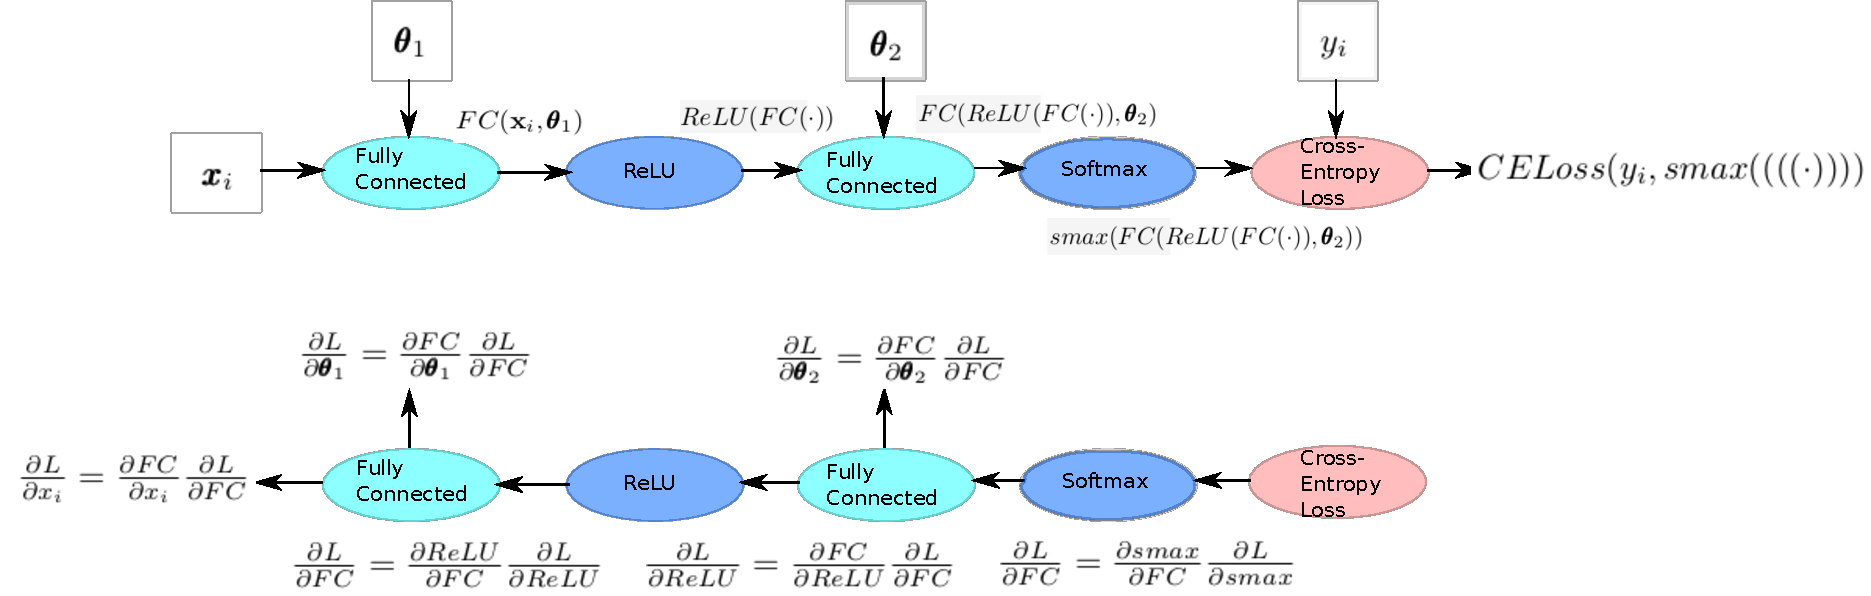
\includegraphics[width=\textwidth]{backprop}
	\caption{A simple example of forward (top) and backward passes (bottom) for a simple two-layer ANN. This illustrates how gradients that flow to early layers are calculated by multiplying the local gradient of a given layer with the gradient that flows back from the upstream layer}
	\label{fig:backprop}
\end{figure}

After gradients have been calculated using back-propagation, they are used by an optimization algorithm to alter the model's parameters, with the aim of minimizing the loss function. Here we consider stochastic gradient descent (SGD) \cite{Robbins1951} which is the most widely used optimization algorithm in deep learning. The algorithm is called stochastic because at each learning iteration only a mini-batch, of the data is use to calculate the gradients. It has been shown that SGD converges much faster than calculating gradients always on all available data; the time per update for the algorithm is independet of data size, as long as the batch size is held constant \cite{Goodfellow2016}. The parameter updates are based on moving 'downhill' i.e. in the direction of negative gradient:

\begin{align} \label{sgd_eq}
  \pmb{\theta}_{(t+1)}=\pmb{\theta}_{(t)} - \eta \nabla_{\theta_{(t)}}L(\mathbf{X}, \mathbf{y})
\end{align}
where $\nabla_{\theta_{(t)}}L(\cdot)$ is the gradient of a loss function with respect to model parameters (multi-variable equivalent of derivative), and $\eta$ is the learning rate.

Most deep learning models are very sensitive to the choice of learning rate. If it is too high, we are likely to miss minima, and conversly there is a risk of local minima and slow training when it is set too small. Usually learning rate is reduced linearly with training time, or in bigger steps at regular intervals. This reduces the impact of noise when we approach a minimum \cite{Goodfellow2016}.

A common addition to the vanilla SGD is momentum \cite{Rumelhart1985}, which can accelerate learning when there is a lot of noise or when the Hessian of the loss (matrix of 2nd order derivatives) is ill-conditioned, as shown in Figure \ref{fig:momentum}. SGD with momentum ammends the original SGD by introducing a velocity term that accumulates gradients from previous iterations with an exponential decay \cite{Goodfellow2016}. Rumelhart and Hinton \cite{Rumelhart1985} described momentum as if dropping a ball-bearing on loss surface and letting gravity accelerate the ball. Further, the loss landscape can be imagined to be immersed in a liquid with a specified level of viscosity that defines how quickly the ball's momentum fades. Algorithm \ref{alg:sgd_mom} gives an example of full SGD momentum algorithm. In practice, backpropagation and SGD-based optimization can nowadays be done automatically in modern deep learning libraries such as PyTorch \cite{Paszke2017} and TensorFlow \cite{Abadi2015}. 

\begin{figure}
  \centering
	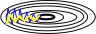
\includegraphics[width=0.5\textwidth]{momentum}
	\caption{Example of an ill conditioned Hessian. Momentum speeds up learning by accumulating the gradients of previous iterations such that velocity towards centre (lower loss) is established (shown in yellow). SGD without momentum keeps jumping across the loss surface as if in a downward sloping canyon, but fails to utilize the slope (blue trace). The contours depict different levels of loss that decreases inwards}
	\label{fig:momentum}
\end{figure}

\begin{algorithm}
  \caption{SGD with momentum (following \cite{Goodfellow2016})} \label{alg:sgd_mom}
\begin{algorithmic}
  \Require Learning rate $\eta$, Momentum decay parameter $\alpha$
  \Require Initial parameters $\pmb{\theta}$, initial velocity $\nu$
  \While{Convergence not met}
  \State Sample a minibatch of m observations from training data $\{\mathbf{x}_1, \dots, \mathbf{x}_m \}$
  \State Get corresponding targets from training data $\{\mathbf{y}_1, \dots, \mathbf{y}_m \}$ 
  \State Compute gradient for the minibatch: $\mathbf{g} \leftarrow \frac{1}{m} \nabla_{\theta}\sum_i L(f(\mathbf{x}_i| \pmb{\theta}), \mathbf{y}_i)$
  \State Update velocity: $\pmb{\nu} \leftarrow \alpha \pmb{\nu} - \eta\mathbf{g}$
  \State Updata parameters: $\pmb{\theta} \leftarrow \pmb{\theta} + \pmb{\nu}$
  \EndWhile
\end{algorithmic}
\end{algorithm}

\subsection{Convolutional Neural Networks (CNNs)}

So far we have considered only simple feedforward ANNs with fully connected layers. Most of the ground-breaking accomplishments over the past decade in deep learning have however been achieved with convolutional neural networks (CNNs) \cite{Le} of some sort. This is particularly true for computer vision tasks such as image classifiction \cite{JurgenSchmidhuber2015}. In fact, the term deep learning is often used synonymously with CNNs that have a large number of layers.

Unlike fully connected neurons in feedforward networks, convolutional layer has neurons, usually called kernels, which are connected only to some parts of the input - together many such neurons span the entire input data. Furthermore, there is weight sharing between the kernels to allow for the recognition of a particular feature anywhere in the input space \cite{Lecun2015}. Convolution layers are therefore particularly suited for data with locally correlated structures such as images. Consider an input image of 225x225, a typical convolution filter may have size 3x3 and, after being trained on the image data, it could have learned to represent a particular visual feature such as a vertical edge. This filter is then replicated over the entire 225x225 input range so that the model can detect vertical edges anywhere in the image. Usually each layer has a multitude of kernels that are able to detect different features. Mathematically, this feature detection corresponds to the convolution operation between input data $X$ and convolution kernels $K$,. For discrete 2D data  this is given as $S(i, j) = (X \ast K)=(i, j) \sum_m \sum_n X(i-m, j-n)K(m, n)$ \cite{Goodfellow2016} where $i$ and $j$ denotes a particular pixel location and $m$ and $n$ the location in the kernel layer. Figure \ref{fig:conv} gives a brief toy example to illustrate this process. 
  
\begin{figure}
  \centering
	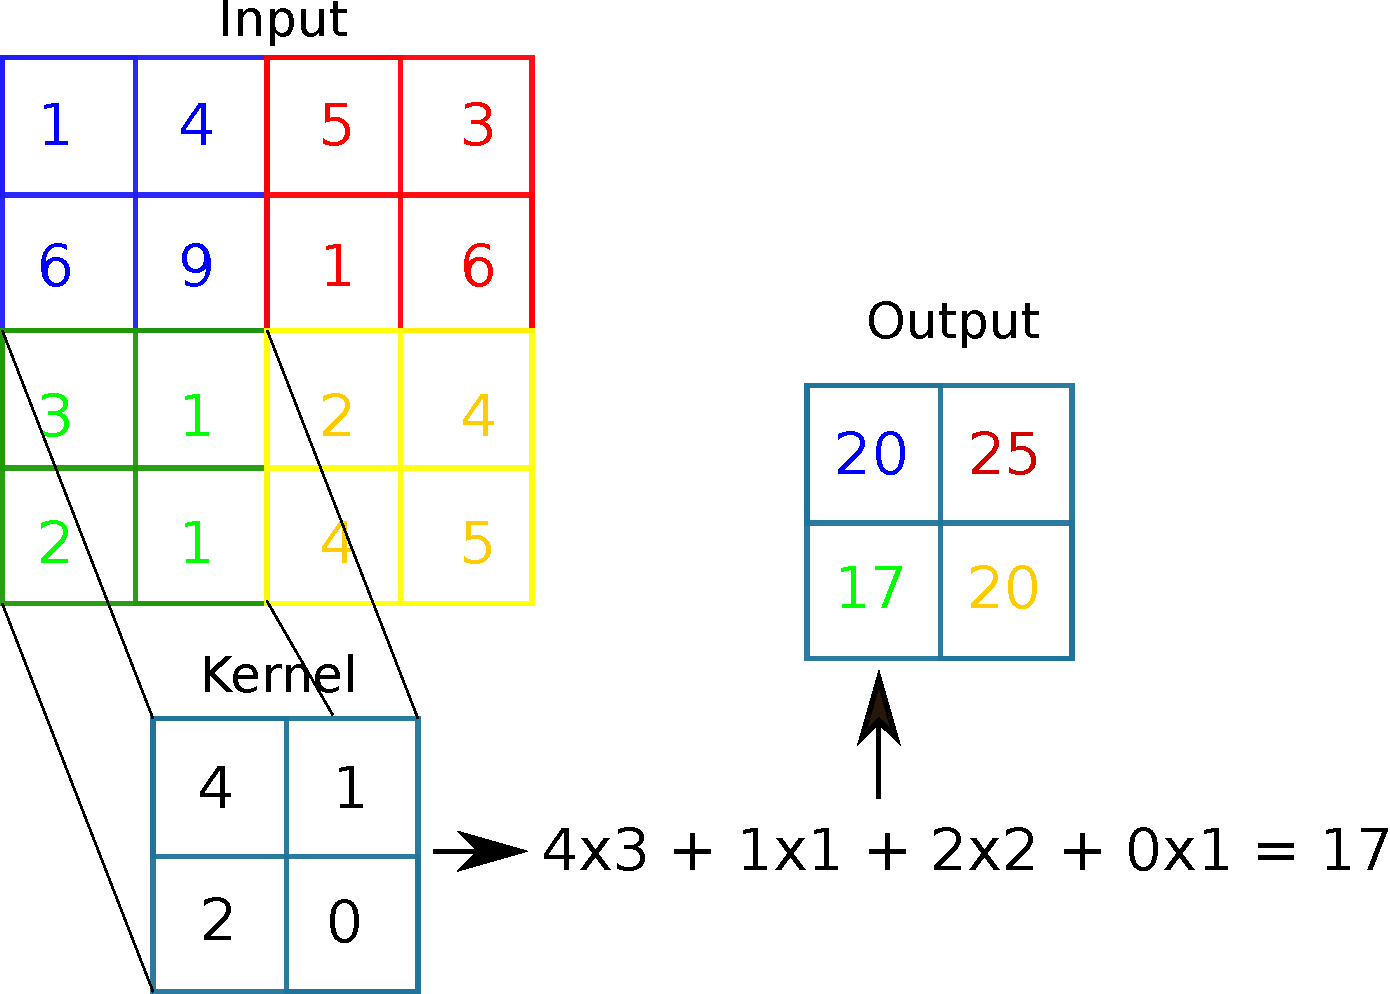
\includegraphics[width=0.7\textwidth]{conv}
	\caption{A simple example of the computations performed by a single 2x2 convolution kernel on a 4x4 input. Assuming stride length of two squares, the kernel will see each of the four corners and performs a convolution operation on each of them. This is shown explicitly for the bottom left green square. The computation is hence essentially a dot product similarity metric between the kernel and the local image areas.}
	\label{fig:conv}
\end{figure}

The reason why convolutions have proven so effective for image data is that natural visual scenes present strong local correlations - the world we view is not just a collection of randomly ordered pixels. Additionally, visual features can appear anywhere in our visual field; thus the need for convolution layers to scan across the whole image \cite{Lecun2015}. Further, CNNs usually have several layers of convolutions on top of each other. When such deep CNNs are trained on image data, the kernels across the different layers usually learn a hierarchy of visual features: the early layers detect edges and corners, which are then used by middle layers to create contours and parts of objects, and finally later layers build up more complex representations, possibly of complete objects \cite{Zeiler2014}. This shares some similarities with the mammalian visual cortex \cite{Cadieu2014} in which earlier (V1) cells respond to edges and bars of different orientations \cite{Hubeld1962} and later ones, like V4 and the IT cortex, to more complex shapes \cite{Kobatake1994}. 

Convolution layers in CNNs are normally followed up by max-pooling functions. Usually these come in the form of the $max()$ functions applied on top of convolution outputs. For example, in Figure \ref{fig:conv} a max-pooling operation would only pass through the value of 25. The benefit of such down-samplign is local invariance: visual objects are not completely rigid (imagine a letter that's slightly rotated between different views). By passing on only the largest value, we are likely to produce the same output even if pixel values of the input moved around a bit \cite{Lecun2015}.

One of the most fundamental properties of CNNs is that they can be trained end-to-end using back-propagation and SGD. A very important consequence is that the models automatically learn features that best fit the input data. This dispenses with the need to manually engineer visually features, which was the approach taken by earlir machine vision algorithms such as SIFT \cite{Lowe1999}. CNNs trained on backpropagation produced very large accuracy gains over these methods \cite{Razavian2014}, and following the breakthrough performance of the seminal AlexNet CNN \cite{Krizhevsky2012}, deep CNNs of various designs have become state-of-the-art in virtually all machine vision classification and detection tasks \cite{JurgenSchmidhuber2015}.

Different architectural desings can have a large impact on how well a CNN performs at a given task. For example, deep networks with a large number of convolution and pooling layers have been found to perform better \cite{Srivastava2015} than shallow ones. This is exploited by several CNN models such as the ResNet architectures which can have more than 100 layers \cite{He2015}. Theoretically, depth increases the representational capacity of the network \cite{Sun2015}. Representational capacity is also increased by the use of ReLUs on top of convolution layers. In order to map feature representations into a vector of class predictions, usually the final layer of a CNN contains similar fully-connected layer as feedforward networks.

Modern deep CNNs can easily have hundres of millions of parameters and have recently started to match human performance on many image classification tasks \cite{Lecun2015}. Owing to their large representational capacity, these models can also easily overfit training data. The development of appropriate regularization techniques has thus played a large role in CNNs' success. Perhaps the most popular regularization technique, and the one applied in this work, is \textit{dropout} \cite{Srivastava2014}. At every training iteration, dropout deactivates each neuron with a user-specified probability. As a consequence, training is essentially done over exponentially many different sub-models, and the final model is their average \cite{Goodfellow2016}. This method regularizes the network as individual neurons cannot rely too much on other neurons. At test-time, dropout is turned off.

Many of the theoretical concepts of modern deep CNNs have been around for several decades \cite{JurgenSchmidhuber2015}. The reason for their recent surge in popularity is to a large extent that modern computer resources have made them a lot easier and faster to train. In particular, the ability to train deep models on Graphical Processing Units (GPUs) has cut training times by at least an order of magnitude \cite{Lecun2015}. However, we have only been able reap the benefits of faster compute and better models because of larger datasets. It has been suggested that CNNs with around 5000 labels per training category can on average start to equal human performance on image classification \cite{Goodfellow2016}. Over the past decade we have seen the advent of datasets that have up to tens of millions images on tens of thousands training classes \cite{Russakovsky2015i}, \cite{JiaDeng2009}, \cite{Netzer2011}.

\section{Exploiting Semantic Information in \\ Computer Vision}

\subsection{Semantic Hierarchies and \\ the Human Visual System}
Upon observing almost any visual scene, humans are able to effortlessly cut it up into segments of distinct objects \cite{Rosch1976}, even if we have never seen the scene before. This is a remarkable ability considering that the world we live in can present us with an infinite amount of visual variation to our retinas. Yet we are able to easily recognize tens of thousands of distinct object categories \cite{Biederman1989} with invariance to various factors such as movement, lighting, shade, orientation and partial occlusion \cite{DiCarlo2012}. Rosch \textit{et al.} \cite{Rosch1976} argue that this is because of the non-random, and hierarchical, structure of visual objects, for instance no breed of dogs has wings but they will often share many features such as four legs, snout and a tail amongst each other. In general entities that are closer to each other in a hierarchical semantic taxonomy will typically share more visual features: dogs and birds are still more alike than dogs and vehicles since both belong to a higher level category of animals which all share certain visual attributes. These observations are also corroborated by the importance of physical features in the organisation of hierarchical biological taxa \cite{Ohl2015}.

Standard machine learning and deep learning models used for image classification do not fully exploit this semantic taxonomy since they are trained against one-hot encoded target vectors. For example, the 1K ImageNet data set \cite{JiaDeng2009} will have labels as 1000-dimensional vectors where there is a 1 for the dimension indicating the correct class and 0s elsewhere. It follows that label vectors for different classes are orthogonal, and a model trained on them will not account for any classes belonging to a common category at a higher level of a taxonomy. For example, in reality wolves and dogs fall under the same higher level categories of canines, animals, mammals and so forth - all of these share certain amount of visual features. The chosen level of hierarchy of a one-hot encoding is also usually arbitrary; should an image be labelled a dog or a labrador retriever? Optimally both would be taken into account, we argue. The number of machine learning algorithms that do take this into account is limited, however; below we give an overview of them.

\subsection{Semantic Hierarchies for Image Classification}
The use of semantic hierarchies in computer vision dates back to early work on image retrieval \cite{Aslandogan1997}, \cite{Zhao2001}, \cite{Grosky2002} \cite{Barnard2001}, where they have been used to expand potential query terms and to impose a more general association between image features and corresonding labels. These ideas were subsequently utilized to improve image annotation and classification \cite{Srikanth2005}, \cite{Marszaek2007} \cite{Griffin2013}. For example, Marszalek and Schmid \cite{Marszaek2007} used the WordNet database \cite{Miller1995} to create a lexical hierarchy of their image labels and trained a separate binary SVM classifier \cite{Scholkopf2002} for each node of the hierarchy. The resulting model proves flexible and performs well under uncertainty - if the model is unsure about which dog breed is in an image, it can then move up one level and just predict a 'dog'. The dataset used by the authors is very simple by today's standards, however, and would be difficult to scale up. More recently, Redmon and Farhadi \cite{Redmon} employed a similar idea but in the context of deep learning. In particular, the label for each image was taken to be the full path from the root node of the WordNet tree to the original label. The model was then trained with multiple softmax functions, one for each level of hierarchy, in order produce a chain of conditional probabilities from the root node to leaves. The authors' purpose for building this model was to learn simultaneously from two datasets of unequal hierarchies and to jointly optimize classification and detection on the two datasets. However, other possible benefits, like zero-shot learning, were not explored. 

In their research on human categorization, Rosch \textit{et al.} \cite{Rosch1976} defined the concept of 'basic level'. This is described as the most fundamental level in the semantic hierarchy of visual objects; it is the level that children usually learn first, and humans tend to identify objects most readily at this level. The level below the basic level is called 'subordinate level'. An example of this structure would be the basic level label of 'fox' and its subordinate 'arctic fox'. The importance of the basic level seems to stem from this level having the highest ratio of visual variation between categories to variation within categories \cite{Rosch1976}, \cite{Joliceur1984}. Therefore, it has been especially practical for humans to identify and label objects at this level \cite{Joliceur1984}. 

Hillel and Weinshall \cite{Hillel2007} mimicked the idea of basic and subordinate levels by building a two-stage classifier where the first stage generates a vector representing the different parts of an objects and the second stage classifies instances based on this vector. On average, this strategy outperformed a traditional one-step algorithm. Wang and Cottrell \cite{Wang2015} took these ideas to the deep learning-era, and trained a CNN on both, basic and subordinate, labels of the ImageNet 2012 data \cite{Russakovsky2015}. They found that this increased the standard top-5 classification accuracy. Another simiar study \cite{Lei2018} explored a dataset which mostly had coarse labeled images (akin to the basic level) and only some fine grained examples. The authors showed that training at both of the two levels helped to predict the fine-level classes. This suggests that the fine-grained model is able to borrow strength from the coarse labels and subsequently generalize better. Peterson \textit{et al.} \cite{Peterson2018} extended this line of research by exploring the type of representations learned by a CNN trained on both 'basic' and 'sub-ordinate' labels. First, the authors found that including basic-level labels in pre-training led to a much more clustered representation of the CNN features, e.g. the feature vectors of different breeds of dogs were now bundeled up together. They also illustrated the generalization power of these representations by running a few-shot learning experiment in which the model was shown only a handful of examples of either sub- or basic-level objects. Zero-shot learning was not considered however. All of the above works have only considered hierarchies of few levels; we are not aware of any deep learning papers that would have explored the type of representations and the consequent generalization properties that would result from using a more complex hierarchy of labels.

\subsection{Semantic Embeddings and Zero-shot Learning} \label{sec:semlit}
Above studies illustrate the implicit connection between semantic and visual data processing in humans. Joliceur \textit{et al.} \cite{Joliceur1984} explored this in depth and illustrated these capabilities with several experiments. For instance, upon viewing a picture of a chair, we can use our semantic knowledge-base to generalize it to the category of furniture even though the image itself doesn't reveal that such a category even exists. Similarly, we can seamlessly access our visual memory to imagine concepts, even ones we may have never seen such as a 'cat wearing ice skates'. If we encounter an uknown dog breed, we are conscious of the uncertainty and will not try to claim that it is a labrador retriever, instead we might say it's some sort of a dog that is similar to a labrador. Or if we are completely unsure, we can just say that it's a dog. We are thus able to perform robust inference on previously unseen classes of objects.

Zero-shot learning (ZSL) \cite{Palatucci2009} is concerned with making predictions about previously unseen classes of images. Formally, a classifier $g$ is trained on features $X_{TR}$ and training labels $Y_{TR}$ such that $g:X_{TR} \rightarrow Y_{TR}$. ZSL requires that $Y_{TR} \cap Y_{ZSL} = \emptyset$ where $Y_{ZSL}$ represents the test labels of any ZSL dataset; training and test labels are completely disjoint. A fundamental idea in this area is to exploit the semantic relatedness of visually linked categories \cite{Monay2004}, \cite{Weston2010}, \cite{Palatucci2009} by projecting input data into a lower dimensional semantic embedding space. This approach can be represented by the following equations \cite{Palatucci2009} (see Figure \ref{fig:zsl} for a graphical explanation):
\begin{align} \label{zsl_eq}
  \mathcal{S} &: X^d \rightarrow F^P \\
  \mathcal{L} &: F^P \rightarrow Y
\end{align}
where $X^d$ is the $d$-dimensional input space, $F^P$ a $P$-dimensional embedding space, $Y$ the class-label space, and $\mathcal{L}$ is a look-up table between embedding vectors and their class labels.

Further, assume that we have all the pairs $\{\mathbf{f}, y\}_{1:M} \in F^P \times Y$ for both the training and zero-shot classes, total $M$ classes. In the training-phase of zero-shot learning, there are $N$ training pairs $\{\mathbf{x}, y\}_{1:N}$, where $N<<M$. Since each $y$ has a corresponding embedding vector $\mathbf{f}$, a classifier $g(\cdot)$ can be trained on $\{\mathbf{x}, \mathbf{f}\}_{1:N}$ to approximate the mapping $\mathcal{S}$. After training, zero-shot prediction can be done by first mapping all the test images $\{\mathbf{x}\}_{(N+1):M}$ into the embedding space:
\begin{align}
\mathbf{\hat{f}}_i = g(\mathbf{x}_i)\,\,\forall i \in (M+1):N
\end{align}
Next, a nearest neighbour classifier $nn$ can be utilized to assign a ground-truth embedding to the predicted embeddings: $nn:\mathbf{\hat{f}} \rightarrow \mathbf{f}$ and subsequently $\mathcal{L}$ is used to get the predicted class labels. To be clear, the term 'zero-shot' refers to the previously unseen $M-N$ classes of test images, however, in our semantic knowledge-base we do know about the existence of those classes and their names. The challenge is thus in how to construct the semantic embedding space and what type of classifier to use to approximate $\mathcal{S}$; the following paragraphs will cover the existing approaches.

\begin{figure}
  \centering
	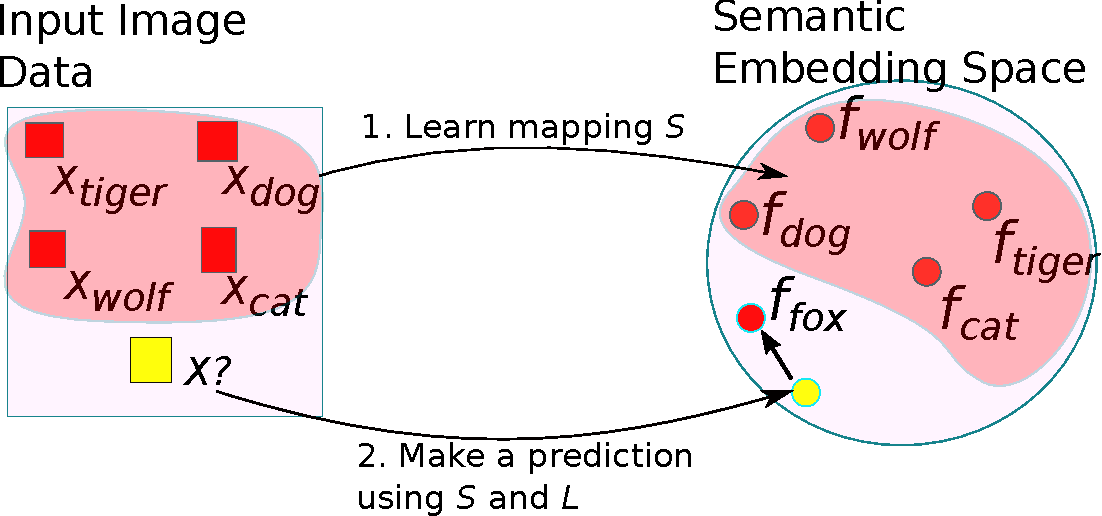
\includegraphics[width=\textwidth]{zsl}
	\caption{A graphical illustration of zero-shot learning. The left square contains all the input images. Red ones are training classes which are used to learn an approximation of the mapping $\mathcal{S}:X^d \rightarrow F^P$. The circle represents the semantic embedding space. Note that embedding vectors for zero-shot classes can be accessed as well. Upon seeing an image of unknown class (yellow square) the model outputs embedding vector prediction (yellow dot) and then the nearest plausible class (here fox) is found with a nearest neighbor function $\mathcal{L}$. Novel image is hence classified as a fox even though the model has never seen one before}
	\label{fig:zsl}
\end{figure}

In an early work, Socher \textit{et al.} \cite{Socher} created word embedding vectors for all seen and unseen class labels from the Wikipedia text data using a methodology \cite{Huang2012} that places words that occur in a similar context next to each other in the embedding space. A two-layer feedforward network was used to learn a mapping from image features into the embedding space, and outlier detection was used to determine if the predicted embedding was one of the known or unknown classes. Only 8 known classes and 2 unknown classes were considered however. To address this and other limitations, Frome \textit{et al.} \cite{Frome2013} developed the Deep Visual-Semantic Embedding Model (DeViSE), which was trained on 1000 classes of the ImageNet dataset \cite{JiaDeng2009} and its zero-shot recognition abilities were tested on the remaining 21,000 ImageNet classes. The architecture of this model forms the foundation for the model we build in this paper: it takes a pre-trained deep learning model, AlexNet \cite{Krizhevsky2012}, removes the softmax layer and replaces it with a projection layer that attempts to predict the embedding vector of each image label. The word embeddings were extracted with another similarity-based model, word2vec, trained on 5.4billion words of text from Wikipedia \cite{Mikolov2013}, \cite{Mikolov}. 

The authors of DeViSE worried, however, that the model was overfitting the projection from the image space into the semantic embedding space. To overcome this they introduced another model, ConSE \cite{Norouzi2013}. In this model, an image of unknown class is first passed into a pretrained CNN. The CNN will try to classify the image as one of the known classes and outputs corresponding label probabilities, $p_0 (y | \mathbf{x})$ such that $\sum_{y=1}^{n_{seen}} p_0 (y | \mathbf{x}) = 1$. The predicted semantic embeddings for the zero-shot images are computed as a convex combination of the known classes' embedding vectors, weighted by the predicted probabilities from the previous step. More formally \cite{Norouzi2013}:
\begin{align}
  f(x) = \frac{1}{Z}\sum_{t=1}^T p(\hat{y}(\mathbf{x}, t)| \mathbf{x}) \cdot \mathcal{G}(\hat{y}(\mathbf{x}, t))
\end{align}
where $\hat{y}(\mathbf{x}, t)$ is the $t^{th}$ most likely class-label for image $\mathbf{x}$ out of the known labels, with $p()$ giving the respective predicted probabilities. $\mathcal{G}$ denotes a look-up table that maps labels to their embedding vectors. $Z$ is a normalizing consant, and $T$ is user-defined. This model was shown to generalize slightly better to zero-shot classes than DeViSE. One contribution of this thesis is to show how the ConSE model can be adapted into hyperbolic space.

A potential problem with the above models, which use Wikipedia text data to create semantic embeddings, is that vectors for low occurence labels may be imprecise. Li \textit{et al.} \cite{Li2015} attempted to resolve this by exploiting the full WordNet semantic hierarchy \cite{Miller1995}. To do this, they re-constructed the semantic embedding for each word by tracing its path to the root of the WordNet tree and calculated an inverse distance-weighted combination of the Wikipedia-based semantic embeddings along the path. For example, the embedding vector for 'arctic fox' was constructed as a combination of the word2vec semantic embeddings of the set ('arctic fox', 'fox', 'canine', 'carnivore' \dots 'living being'). Despite the attempt to capture the semantic structure of the WordNet, the embeddings at each node are still based on the Wikipedia data, which does not account for this taxonomic structure. Further, each label only considers its own parent super-ordinate nodes. Consequently the resulting embedding manifold as a whole is sparse and hence unlikely to accurately reflect the full WordNet graph and its complex relations. In the next section we show how this has recently been achieved with hyperbolic embeddings.

Fu \textit{et al.} \cite{Fu2015} identified a central issue that maligns most ZSL approaches, namely the projection domain shift: the mapping that is learned from the training image space into the embedding space may not transfer well to the disjoint set of zero-shot classes. Transductive multi-view embedding was proposed as a solution by the authors: in addition to the semantic embeddings of the seen classes, the embeddings of unseen classes are also available and can hence be used at training time. In fact, multiple embeddings for each label were created and they were all jointly projected to common embedding space, which alleviated the domain shift problem. Kodirov \textit{et al.} \cite{Kodirov2015} proposed a similar approach: sparse coding was used to map from the unseen labels to the semantic space. This helped to guide the domain projection from seen to unseen visual features. See also Rohrbach \textit{et al.} for similar ideas \cite{Rohrbach2013}. The use of test labels during training may not be practical, however, and as an alternative Kodirov \textit{et al.} \cite{Kodirov2017} proposed a semantic autoencoder. The general idea is to learn one mapping (decoder) from input images to a latent semantic embedding space and another mapping (decoder) from there back to reconstruct the image data. The addition of the decoder constraints the model to solve the domain shift. Tsai \textit{et al.} \cite{Tsai2016} used two autoencoders, one on the image data and another on text data, extracted the representation layer from each and minimized their mismatch. 

Several other approaches have been suggested for learning the mapping from image data into the embedding space. For example, Fu and Sigal \cite{Fu2016} used embeddings built on full semantic vocabularies, rather than just training labels, and showed that a better mapping was learnt. Shigeto \textit{et al.} \cite{Shigeto2015}, on the other hand, showed that instead of learning a mapping from image data into the label space, it can be beneficial to go in the opposite direction since nearest neighbor search is often easier in the lower dimensional image space. Changpinyo \textit{et al.} \cite{Changpinyo2017} also based their models around this idea, with impressive results. Finding nearest neighbours in high dimensional spaces is a common challenge with Euclidean spaces, which we manage to avoid by working in low-dimensional hyperbolic geometry instead.

Another branch of works has focused on learning better embeddings. While most approaches learn a semantic embedding and the mapping function separately, Ba \textit{et al.} \cite{Ba2015} trained a feedforward network from text input data to predict the visual features in the different layers of a CNN. Together these networks defined a joint-embedding, which was shown to capture fine-grained visual features more accurately. Ji \textit{et al.} \cite{Ji2017} showed how performance can be improved by ensuring that the embedding manifold preserves the local structure of the visual input space. Local similarity aware deep embeddings were explored by Huang \textit{et al.} \cite{Huang2016}. Zhang and Saligrama \cite{Zhang2015}, on the other hand, built semantic embedding labels for zero-shot classes as mixture distributions of the seen classes' embedding vectors. In a follow up work the authors \cite{Zhang2015a} provided a latent probabilistic framework; that is, zero-shot recognition is performed by estimating the posterior probability that an image matches one of the label vectors. 

Graph-based approaches have also been popular in tackling ZSL recently \cite{Fu2015a, Changpinyo2016, Wang2018a}. Most notably, the current state-of-the-art \cite{Wang2018a} exploits both, explicit taxonomic relationships between categories from the WordNet graph, as well as similarity based semantic embeddings constructed from the Wikipedia text data \cite{Pennington2014}. More specifically, each node in the WordNet graph is replaced by its respective semantic embedding vector. A \textit{graph convolutional network}, which performs convolutions between the nodes, is used to predict logistic regressors that are used for zero-shot recognition. The results of the this current state-of-the-art approach highlight the difficulty of the ZSL task: they achieve around 2 \% top-1 accuracy and 12 \% top-20 accuracy on predicting labels for 21k zero-shot classes. The approach taken by the authors is similar to ours in that they also try to explicitly represent semantic hierarchies, as well as similarities, however in our work both are captured by the embedding space. Further, our approach has the advantage that it can be combined with standard deep learning models, which is important given their ubiquity.

In addition to above, there is a vast array of approaches that focus on zero-shot learning via class attributes \cite{Farhadi2010}, \cite{Rohrbach2010}, \cite{Rohrbach2011}, \cite{Hwang2014}, \cite{Akata2016}, \cite{Xian2016}, \cite{Romera-Paredes2017}, \cite{Bucher2016}. A limitation of these approaches is that when the number of classes grows very big, it becomes harder to manage the space of attributes manually. The set of attributes is also hard to transfer into a new context \cite{Ba2014} with different attributes. Therefore our work focuses solely on text and language based semantic embeddings. More importantly, attribute based ZSL often aims to predict fine-grained classes that are visually very similar \cite{Xian2016} \cite{Reed2016}. We on the other hand aim to build a framework that makes semantically robust zero-shot classifications, such as predicting a higher-level category when the model is uncertain.

Finally, there exist various studies that combine language and attribute based semantic embeddings \cite{Akata2015}, \cite{Fu2015} \cite{Zhou2005}. Akata \textit{et al.} \cite{Akata2015}, for instance, combine three embeddings, one learned from the Wikipedia dataset, one from physical attributes of animals, and a hierarchical embedding based on the structure of the WordNet. The model performs well on zero-shot prediction of fine-grained classes on a relatively small data set; it's generalization properties on a large dataset such as the 21k label ImageNet is not explored, however. A more comprehensive review of further ZSL approaches and trends can be found in \cite{Xian2017}.


\section{Semantic Embeddings in Hyperbolic Space}

\textbf{Section overview:} As alluded to in the previous section, hyperbolic spaces provide an efficient way of embedding hierarchical graph structres. In this chapter we provide a brief overview of the required theoretical background and discuss the recent literature on building word embeddings in this space. Hyperbolic geometry and hyperbolic spaces are a vast fields containing thousands of years of work and formal statements and proofs are thus out of the scope of this work; we merely aim to provide the background necessary for the present work. For more thorough treatment of the topic, we refer the reader to Cannon \textit{et al.} \cite{} and Greenberg \cite{Greenberg1994}; unless where otherwise stated, all the theories and intuitions provided below are based on these two books.

\subsection{Basics of Hyperbolic Geometry}
Hyperbolic geometry is a type of non-Euclidean geometry, derived by altering the fifth postulate of the classic Euclidean geometry \cite{Greenberg1994}:
\begin{enumerate}
    \item Any pair of points can be joined up by stricly one staight line segment
    \item All lines can be extended indefinitely
    \item Exactly one circle of a specific circle and specific centre exists
    \item All righ angles are identical
    \item Parallel postulate: Consider line L and a point P which does \textit{not} lie on L. Then there exists only one other line M that passes through P and is parallel to L, no matter how much we extend the two lines.
\end{enumerate}

In hyperbolic geometry the fifth postulate becomes its negation: 

\begin{enumerate}
   \setcounter{enumi}{4}
   \item * Consider line L and a point P which does \textit{not} lie on L. For any L, there are infinitely many lines that are both parallel to L and pass through P.
 \end{enumerate}

\begin{figure}
  \centering
	\includegraphics[width=0.5\textwidth]{pdisklines}
	\caption{Parallel lines in Hyperbolic space (Poincare disk model). The thick blue line is parallel to all the other lines since it never intersects any of them in the hyperbolic space (interior of the circle). All the lines are arcs of circles of different sizes that fall in the interior - these are known as geodesics. Image used under Creative Commons license, released into public domain by Trevorgoodchild of English Wikipedia}
	\label{fig:disklines}
\end{figure}

\begin{figure}
  \centering
	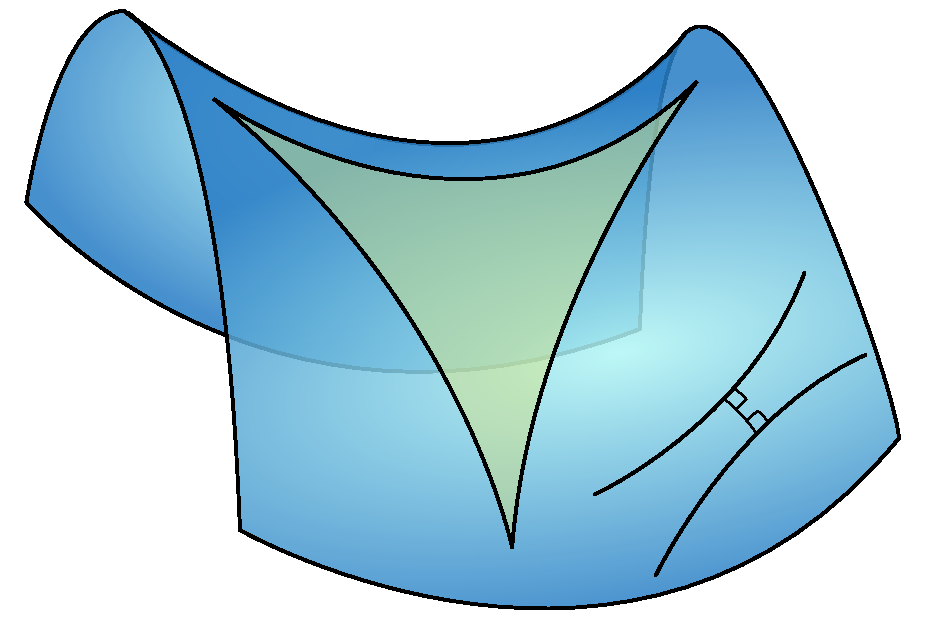
\includegraphics[width=0.5\textwidth]{hsaddle}
	\caption{Saddle point in Euclidean space allows a representation of a hyperbolic triangle, for which the sum of its angles is less than 180 degrees. Image used under Creative Commons license from Wikimedia Commons.}
	\label{fig:hsaddle}
\end{figure}

For us who are accustomed to thinking in Euclidean terms, this may seem impossible, at first. This becomes possible when we consider spaces of constant negative Gaussian curvature, which indeed is the fundamental property of hyperbolic spaces (Figure \ref{fig:disklines}). For instance a hyperbolic plane is a 2-dimensional manifold with a constant negative curvature; similar logic holds in higher dimensions too \cite{Stillwell1991}. As long as lines in hyperbolic space never intersect each other, they are parallel. Straight lines in hyperbolic space are more precisely known as geodesics - arcs of circle, and locally they define the shortest path between two points in the curved space \cite{Stillwell1991}. It is illustrative to consider the shortest path between two locations on the globe drawn on a flat map, say new york and london; this too is an arc of the great circle of the earth's circumference, rather than a straight line (though in this instance due to a positive curvature). For an improved intuition of hyperbolic geometry, it should be noted that all points in a hyperbolic space can be viewed as saddle points of Euclidean geometry (Figure \ref{fig:hsaddle}). There are several ways of constructing hyperbolic spaces from Euclidean geometry; the only requirement is that aforementioned necessary axioms are satisfied. Below we define the most important models, following \cite{Greenberg1994}.

\subsubsection{The Beltrami-Klein Model}
Consider a circle $\gamma$ of the Euclidean plane, its centre $O$, and radius $OR$ (see Figure \ref{fig:klein}). The hypebolic space is then defined as the interior of all points $X$ for which $OX < OR$ \cite{Greenberg1994}. Lines in the Klein model of hyperbolic space are open chords of $\gamma$, with open referring to a chord without its end points. This model satisfies the requirement of hyperbolic space since if there is a line $l$ and a point \textit{not} on it, $P$, then there are infinite number of parallel lines of $l$ that go through $P$. An example is given in Figure \ref{fig:klein}. The reason why $m$ and $n$ are parallel to $l$ in this figure is that they are open chords in $\gamma$ and at no point of this space do they interect $l$, which is the working definition of parallelism \cite{Greenberg1994}. It is crucial to notice that only the interior of the circle forms the hyperbolic space and the boundary can never be reached, hence the \textit{open} chords as lines. This, combined with the requirement that lines can be extended indefinitely, means that one can get arbitrarily close to the boundary of the circle but never reach it. As a consequences, the distance between two points on the line grows exponentially the further away from the centre we get and therefore we cannot use Euclidean distance (which is not visibly evident from the figures) \cite{Greenberg1994}. Notice also that the appearance of lines as 'straight' is just a matter of mapping them from geodesics \cite{Greenberg1994}, such as those in Figure \ref{fig:disklines}. 

\begin{figure}
  \centering
	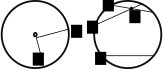
\includegraphics[width=0.6\textwidth]{klein}
	\caption{Depiction of the Klein model of hyperbolic geometry. $m$, and $n$ are parallel lines to $l$ as they never intersect it.}
	\label{fig:klein}
\end{figure}

We can extend this model to any higher dimension $n$ by re-defining the disk as $\mathcal{K}^n = \{\mathbf{x} \in \mathbb{R}^n | \lVert \mathbf{x} \rVert <1 \}$, and taking all other axioms from above. Distance between two points $\mathbf{p}$ and $\mathbf{q}$ is defined as \cite{Iversen1992}:
\begin{align}
  \mathcal{D_K}(\mathbf{p}, \mathbf{q}) = \text{arcosh} \left( \frac{1 - \mathbf{p} \cdot \mathbf{q}}{\sqrt{1-\mathbf{p}\cdot \mathbf{p}}\sqrt{1-\mathbf{q}\cdot \mathbf{q}}}   \right) 
\end{align}

\subsubsection{The Poincare Model}
In the Klein model arcs were mapped to straight lines. An alternative representation of hyperbolic space is the Poincare model. Here two types of lines exist: open chords that pass through the origin of the circle, which are like those in the Klein model, and arcs of all the circles orthogonal to $\gamma$ i.e. \textit{open} arcs (Figure \ref{fig:pdisk}) \cite{Greenberg1994}. The other statements about Klein model transfer here; the boundary can never be reached and distances grow exponentially as we approach it. Again an infinite number of parallel lines exist. This is visualized in Figure \ref{fig:disklines}.

\begin{figure}
  \centering
	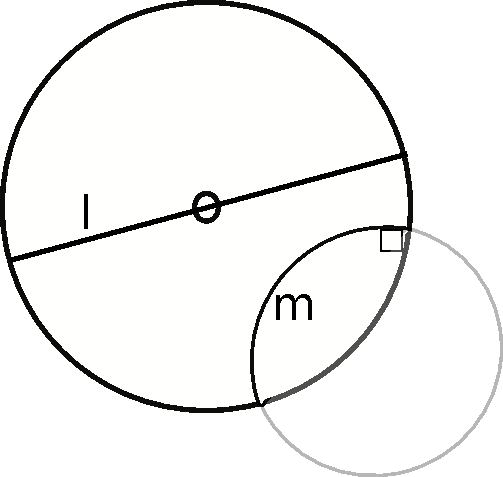
\includegraphics[width=0.4\textwidth]{poincdisk}
	\caption{Depiction of the Poincare Disk model of hyperbolic geometry. Line $l$ represents an open chord passing through the centre of the circle, whilst line $m$ is an open arc.}
	\label{fig:pdisk}
\end{figure}

To extend this formally into $n$ higher dimensions we can define the hyperbolic space as an open unit ball $\mathcal{B}^n$ as we did for the Klein model $\mathcal{B}^n = \{\mathbf{x} \in \mathbb{R}^n | \lVert \mathbf{x} \rVert <1 \}$, but as straight lines are arcs, we have a different distance function \cite{Iversen1992}:
\begin{align}
  \mathcal{D_P}(\mathbf{p}, \mathbf{q}) = \text{arcosh} \left(1 + 2 \frac{\lVert \mathbf{p} - \mathbf{q} \rVert^2}{(1-\lVert \mathbf{p}\rVert^2)(1-\lVert \mathbf{q}\rVert^2)}   \right) 
  \label{eq:pdist}
\end{align}

Whilst the Klein and Poincare models appear different, they both obey all the same axioms of hyperbolic spaces, in fact, the models are \textit{isomorphic}: there is a one-to-one corresondence between all the points $P$ and $P'$ of the two models, as well as one-to-one correspondence between lines $l$ and $l'$, such that '$P$ lies on $l$ if and only if $P'$ lies on $l''$ \cite{Greenberg1994}. It can be proven that all models of hyperbolic geometry are isomorphic \cite{Greenberg1994}. Therefore it is possible map from one model to another. We will employ the mapping from Poincare ball into the Klein model at a later stage and thus present the required equation here \cite{Greenberg1994}:

\begin{align}
  \mathbf{s} = \frac{2\mathbf{u}}{1 + \lVert \mathbf{u} \rVert^2}
  \label{eq:p2k}
\end{align}
where $\mathbf{s}$ is the point in the coordinates of the Klein model and $\mathbf{u}$ in the Poincare model.

\subsubsection{The Hyperboloid Model}
This model stems from the theory of special relativity. If we denote $x$, $y$ the 2-dimensional coordinates and $t$ as time, then distances are measured by the Minkowski metric \cite{Greenberg1994}:
\begin{align*}
  ds^2 = dx^2 + dy^2 - dt^2
\end{align*}
The surface equation that corresponds to this metric is given by the equation below. See \cite{Greenberg1994} for details.
\begin{align*}
  x^2 + y^2 - t^2 = -1 
\end{align*}

In Euclidean space, this forms a hyperboloid object with two sheets \cite{Greenberg1994}, with the upper sheet shown in Figure \ref{fig:lorenz}. In that figure we also show how the model relates to the Poincare disk we saw above. The 'bowl' of the hyperboloid is infinite so the 'brim' can never be reached, thus satisfying the indefinite extensibility of lines, which are geodesics on the hyperboloid surface.
\begin{figure}
  \centering
	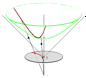
\includegraphics[width=0.6\textwidth]{lorenz}
	\caption{Upper sheet of the hyperboloid model in $\mathbb{R}^3$ and a projection of one of its geodesics on to the Poincare disk. While not possible to visually illustrate, the brim of the 'bowl' is at infinity and can never be reached. Image used under Creative Commons license from Wikimedia Commons.}
	\label{fig:lorenz}
\end{figure}
In higher dimensions, the $n$ dimensional hyperbolic space is defined as $\mathcal{H}^n = \{\mathbf{x} \in \mathbb{R}^{n+1} | \mathbf{x} * \mathbf{x}=-1 \}$ where $\mathbf{x} * \mathbf{x} = \sum_{i=1}^n x_i x_i - x_0 x_0$ is the Lorenzian inner product \cite{Nickel2018} \cite{Cannon}. The distance function is:
\begin{align}
  \mathcal{D_H(\mathbf{p}, \mathbf{q})} = \text{arcosh}(-\mathbf{p} * \mathbf{q})
\end{align}

\begin{figure}
  \centering
	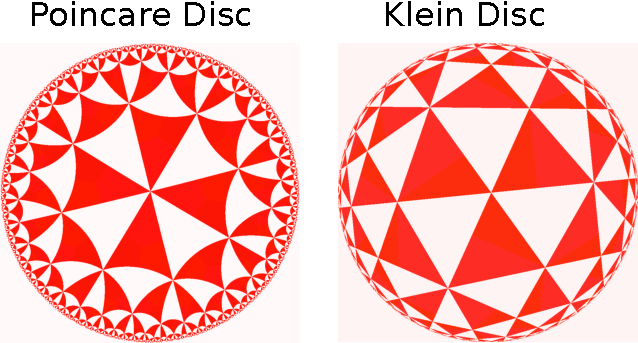
\includegraphics[width=0.6\textwidth]{tiling}
	\caption{Illustrations of Klein and Poincare Disks with hyperbolic tiling. All the tiles have equal area so this visually depicts how the area of the circles grows exponentially towards the boundary. Images used under Creative Commons license from Wikimedia Commons.}
	\label{fig:hyspace}
\end{figure}

\subsection{Semantic Embeddings in Hyperbolic Spaces} \label{sec:poincare}
Most popular word embedding methods take into account the local context of words, e.g. the \textit{word2vec} models \cite{Mikolov, Mikolov2013}, or the global context like the \textit{Glove} model \cite{Pennington2014}, and produce vector representations so that semantically similar words are embedded near each other in the resulting vector space. The ability of these embeddings to capture complex relationships is constrained, however, as the required dimensionality becomes easily exceedingly large \cite{Nickel2017, Chamberlain2017, Nickel2018}. This limit on representational capacity is particularly relevant to our project as we aim to build an embedding space that accurately captures the hierarchical graph structure of word semantics. The idea of using hyperbolic spaces for representing semantic hierarchies more accurately was explored early on by \cite{Ritter1999}, \cite{Ontrup2002} and \cite{Walter2006}, though this was in the context of Self-Organizing Maps rather than word embeddings. More recently, Nickel and Kiela \cite{Nickel2017}, and Chamberlain \textit{et al.} \cite{Chamberlain2017} have succesfully demonstrated the advantages of hyperbolic word embeddings over Euclidean ones in terms of generalization performance and computational cost for representing hierarchical data. Additionally, Gulcehre \textit{et al.} \cite{Gulcehre2018} have achieved success on various tasks, such as neural machine translation, by imposing hyperbolic geometry on the activation functions of their neural network model.

To understand the benefits of hyperbolic word embeddings, consider the Poincare and Klein disk models and contrast this to an Euclidean disk. The area of an Euclidean disk increases quadratically, since $A_E=\pi r^2$, whereas the negative curvature of hypebolic space allows the hyperbolic disk area to grow exponentially with $r$ as given by $A_H=2 \pi \left(\text{cosh}(r) - 1 \right)$ (assuming constant curvature of 1) where cosh is the hyperbolic cosine function $\text{cosh}(x)=\frac{e^{2x} + 1}{2e^x}$ \cite{Greenberg1994}. Intuitively the benefit of this is that in hyperbolic spaces there is much more room for embedding different concepts as we move outwards from the centre (see Figure \ref{fig:hyspace}). Further, Hyperbolic spaces can be interpreted as continuous space extensions of trees and are thus particularly efficient for embedding hierarchical structure in a way that preserves the associated graph structure, even for infinite trees \cite{Chamberlain2017}; like hyperbolic space, the number of leaves of a word-tree also grows exponentially as we increase the levels of hierarchy (assuming the number of splits per level remains constant) \cite{Nickel2017} (See Figure \ref{fig:htree} for a naive example). 

\begin{figure}
  \centering
  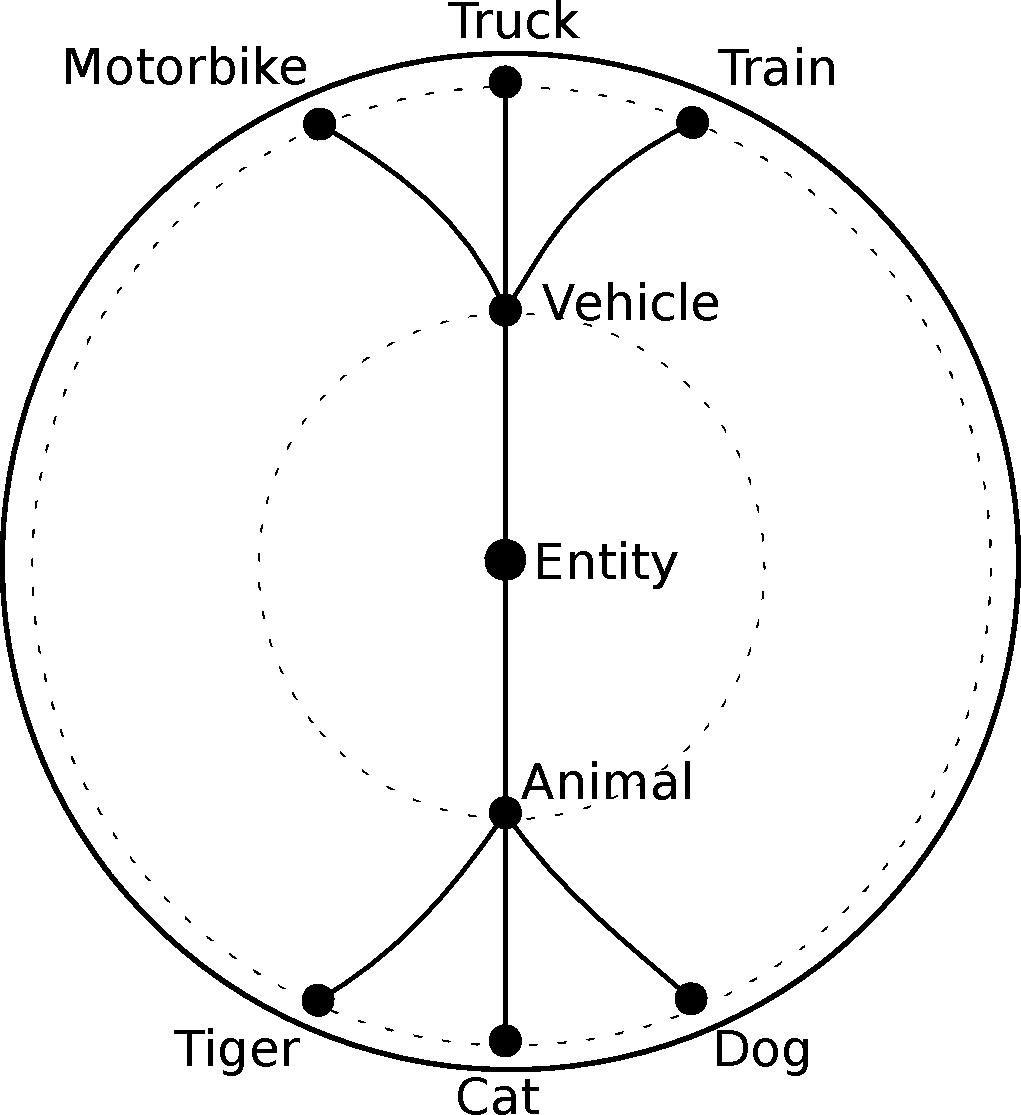
\includegraphics[width=0.6\textwidth]{htree}
	\caption{Naive example of embedding a hierarchical semantic taxonomy in a hyperbolic disk. All the concepts at each level of hierarchy are equidistant from the centre of the disk as portrayed by the dotted circles.}
  \label{fig:htree}
\end{figure}

The hyperbolic embedding that we used is the Poincare Embedding model of Nickel and Kiela \cite{Nickel2017}, mainly because they showed its effectiveness on the Wordnet lexical hierarchy, which is the basis for the labels in the ImageNet dataset that we used. Here we give a brief overview of the way in which the poincare embeddings are actually computed in this model; rest of this section is thus entirely based on \cite{Nickel2017}.  To use the original notation of the paper, let $\mathcal{S} = \{x_i\}_{i=1}^n$ denote the set of words, and $\Theta = \{\boldsymbol{\theta}_i\}_{i=1}^n$ be their repsective locations in the $d$ dimensional Poincare embedding space $\mathcal{P}^d$ i.e. $\boldsymbol{\theta}_i \in \mathcal{P}^d$. To find embeddings, the authors set to solve the following optimization problem:
\begin{align*}
  &\Theta' \leftarrow \text{arg}\,min_{\Theta} \mathcal{L}\left(\Theta\right)\text{  s.t.} \forall \boldsymbol{\theta}_i \in \Theta : \lVert \boldsymbol{\theta}_i \rVert < 1
\end{align*}
where the final inequality is needed to ensure the vectors fall inside the open unit ball. And their loss function is a ranking loss:
\begin{align*}
  &\mathcal{L} \left(\Theta\right) = \sum_{(u,v)} \log \frac{\exp\{-d( \mathbf{u},\mathbf{v})\}}{\sum_{\mathbf{v'}\in N(u)}\exp\{-d(\mathbf{u},\mathbf{v'})\}}
\end{align*}
where the tuple $(u,v)$ represents the nouns that are connected to each other in the WordNet graph, $\mathbf{u}$ and $\mathbf{v}$ are their estimated embedding vectors, and $N(u)$ those nouns $v$ that are \textit{not} connected to a given $u$. Finally, $d(\mathbf{u}, \mathbf{v})$ is the hyperbolic distance betwen the nouns. Since this embedding is based on the Poincare model, the relevant distance function is the one in Equation \ref{eq:pdist}. A point of emphasis is that the model is not given any explicit hierarchical information but can learn it from data on which nouns are connected in the WordNet. It can therefore learn latent hierarchies. 

The optimization problem above could be solved directly using full Riemannian optimization, but the authors show that the Riemanian gradients can also be obtained in terms of Euclidean gradinets $\nabla_E$, resulting in the following Riemannian SGD updates:  
\begin{align*}
  \boldsymbol{\theta}_{t+1} = \text{proj} \left( \boldsymbol{\theta}_t -\eta_t \frac{(1-\lVert\boldsymbol{\theta}_t\rVert^2)^2}{4}\nabla_E \right)
\end{align*}
where $\eta_t$ is the learning rate, and the authords used
\begin{align}
\text{proj}(\boldsymbol{\theta}) = \boldsymbol{\theta}/\lVert \boldsymbol{\theta} \rVert - 10^{-5}\text{ if }\boldsymbol{\theta} \geq 1; \text{ otherwise } \boldsymbol{\theta}
\end{align}
to ensure the updates remain with the open unit ball Poincare space. $\nabla_E$ can be derived using the backpropagation algorithm introduced in Section \ref{sec:trainANN}. This model achieved superior performance in comparison to an Euclidean baseline in various experiments that tested for the models' ability to preserve original graph structures \cite{Nickel2017}.

\subsubsection{Summary of Background}
In this section we have covered the necessary technical background and the most relevant literature that inspired this thesis. Our literature review can be summarized as follow. First, deep learning has achieved unparalleled success in almost all computer vision tasks but in their standard from they are unable to generalize to previously unseen classes. Zero-shot learning tries to address this shortcoming, often by borrowing strength from different forms of semantic embeddings. This is motivated by the observation that semantic similarity often corresponds to visual similarity. Unlike similaritity based embeddings, the human brain categorizes visual objects in a much richer representation of semantic \textit{hierarchies} that allows robust inference on novel objects. We look to replicate this behaviour in the zero-shot setting. Whilst some hierarchical models have been introduced in this area previously, to our knowledge, no work has used the recent hyperbolic embeddings to explore their potential benefits over the standard Euclidean word embeddings.

\chapter{Our Approach}

\section{Approach Overview}
We propose two model architectures Deep Hyperbolic Semantic Embedding (Deep-HSEM) model  and Convex Hyperbolic Semantic Embedding (Convex-HSEM) model . The general intuition is to replace the standard one-hot-encoded targets used in deep learning with poincare embedding vectors that should better reflect the location of each label in a hierarchical semantic taxonomy; we use the lexical database WordNet as the hierarchy \cite{Miller1995}. By training against these hierarchical embedding labels, we exploit the fact that many objects of initially different categories share common visual attributes through a shared super-catgory. For images, we use the ImageNet Large Scale Visual Recognition Challenge (ILSVRC) 2012 1000-class dataset \cite{JiaDeng2009}. After we have learned a mapping from images into the hyperbolic embedding space, we then perform zero-shot recognition by feeding previously unseen classes of images through the trained model and then search for the nearest label in the embedding space. In total we use 20,000 classe of unseen images for the zero-shot evaluation. These images come from the broader 21K full ImageNet 2011 dataset. Crucially, we hypothesized that hyperbolic embedding space which is based on semantic hierarchy will reflect visual similarities better than pure similarity based word embeddings which just captures the context the words occur in; words that occur in a similar context could easily have no visual resemblence. To explore this, we also performed the zero-shot experiment with a version of our model that uses the Glove embedding in place of the hyperbolic embedding.

\section{Model Details}

\subsection{Poincare Embedding Construction}
In order to learn a mapping between images and their location in the hyperbolic embedding space, we first had to acquired the ground truth hyperbolic embedding vector for each image label. Since all of the ImageNet class-labels correspond to specifc words in the WordNet lexical database, WordNet was the obvious choise for based on which to construct the hyperbolic embeddings. Moreover, WordNet provides exactly the type of lexical semantic hierarchy that we were looking to use. As a whole, the WordNet consists of 117,000 synsets (synonym sets; words in a single synset share a meaning), which are connected to each other in a graph based on their super- and sub-ordinate relations. These relations are transitive so that if A is an subordinate of B and B is subordinate of C, then A is also subordinate of C. Several different types of words are encoded in WordNet, such as verbs and nouns. In this work only nouns were considered. One potentail issue was that each synset may contain several nouns, but fortunately the ImageNet database provides an exact mapping from each image class to a specific noun. Overall, our final list consisted of 82,000 of commonly used nouns, including all the 21,000 classes of the full ImageNet. Note that we also used nouns not included in the ImageNet labels in order to learn a more accurate structure for the hyperbolic embedding.

The specific hyperbolic embedding model we used is Poincare embedding model of Nickel and Kiela \cite{Nickel2017}, which was described in detail in Section \ref{sec:poincare}. These authors also provided an open-source implementation of the model \footnote{\label{fb_fn} Available at https://github.com/facebookresearch/poincare-embeddings} , which we used to construct Poincare embeddings for all the 82,000 nouns. The dimensionality of embedding vectors was chosen to be 10 for this project. This is much lower than the number of dimensions usually used by Euclidean word embeddings (50 to 500) and thus allowed us to demonstrate the relative efficacy of hyperbolic embeddings. Further, \cite{Nickel2017} illustrated very good predictive performance for 10 dimensions specifically on WordNet reconstruction. To get our final label embeddings, we trained the Poincare embedding model with default hyperparameters for 1500 epochs (4 days run-time). Important detail of the model is that we only provide it with information about which nounds are connected to each other, that is, no explicit hierarchical relation need to be given to the model, rather the embedding self-organizes to learn the latent hierarchy.

\subsection{Deep Hyperbolic Semantic Embedding Model \\ (Deep-HSEM)}
\subsubsection{Model Architecture}
Typically convolutional neural network takes in an image and outputs predicted probabilities for the different possible class labels. Our model is very similar with the crucial exception that, for each image, Deep-HSEM predicts a single vector that corresponds to a point in the Poincare embedding space. More precisely, we have taken a well known CNN architecture, VGG-16 \cite{Simonyan2014}, and re-adjusted its final output layer by taking out the softmax layer and replace it with a fully connected layer that corresponds to the dimensionality of the Poincare embedding space. We chose the VGG-16
model since it provides near state-of-the-art performance on the ImageNet 2012 1K data (top-1 accuracy 76.3\%, top-5 accuracy 93.8\%) but is simpler and less costly to train than many of the more recent CNNs. The architecture of the VGG-16 consists of 16 layers: 13 3x3 convolution layers followed by three fully-connected layers. Additionally, the network uses 2x2 max-pooling, ReLU non-linearities and dropout for regularization. We illustrate the Deep-HSEM architecture in Figure \ref{fig:dhsem}. The resulting architecture is very similar to the DeViSE model of Frome \textit{et al.} \cite{Frome2013} (reviewed in Section \ref{sec:semlit}); the most significant difference is that our model outputs predictions within the Poincare embedding hyperbolic space. 

\begin{figure}
  \centering
  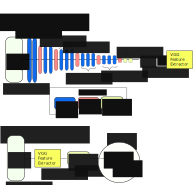
\includegraphics[width=\textwidth]{VGG16}
  \caption{a.) Original VGG-16 structure except that we have taken out the final classification layer. The resulting model extracts 4096 long feature vector from the input image b.) The VGG feature extractor is attached to at fully-connected layer which outputs 10-dimensional embedding vector prediction. The distance of this prediction from the ground-truth embedding vector is used to compute a scalar loss. This is used to backpropagate gradients through the network.}
  \label{fig:dhsem}
\end{figure}

Formally, our aim is to learn a mapping $S$ from 224x224 RGB image space $X^{224x224x3}$ into the 10-dimensional Poincare embedding $F_{\mathcal{P}}^{10}$.
\begin{align*}
\mathcal{S}: X^{224x224x3} \rightarrow F_{\mathcal{P}}^{10}
\end{align*}
In order to learn this mapping, the Deep-HSEM, denote it $h_{deep}(X, \pmb{\theta})$, where $\pmb{\theta}$ denotes the model weights, is provided with training data pairs of input images and corresponding embeddings $\{X, f\}$. The model takes the input image $X$ and predicts an embedding $\hat{f}$:
\begin{align*}
  h_{deep}(X, \pmb{\theta}) = \hat{f}
\end{align*}
The Poincare hyperbolic space in this instance is defined as the 10-dimensional open unit ball:
\begin{align*}
  F_{\mathcal{P}}^{10}=\{\mathbf{f} \in \mathbb{R}^{10} | \lVert \mathbf{f} \rVert <1 \}
\end{align*}
Note that we need to therefore ensure that the Deep-HSEM outputs are constrained into this space. This is ensured by the below operation performed at the end of the network:

\begin{equation}
\mathbf{\hat{f}} =
\begin{cases}
   \frac{\mathbf{\hat{f}}}{\lVert\mathbf{\hat{f}}\rVert}, & \text{if}\ \lVert\mathbf{\hat{f}}\rVert \geq 1 \\
   \mathbf{\hat{f}}, & \text{otherwise} 
\end{cases}
\end{equation}
In order to train the model parameters $\pmb{\theta}$, a loss function $L(\mathbf{\hat{f}}, \mathbf{f})$ was minimized. We considered various alternatives: squared Poincare distance, ranking hinge-loss on Poincare distance, and softmax-cross entropy loss on Poincare distances. The softmax-cross entopy loss was found to perform the best and was used for all the models presented here. In order to adapt the standard cross-entropy softmax (Equation \ref{softmax_eq}) we calculated the Poincare distance $\mathcal{D_{\mathcal{P}}}(\mathbf{\hat{f}}, \mathbf{f}_i)$ (Equation \ref{eq:pdist}) between the predicted embedding and all the possible ground-truth class embeddings. Since we want to minimize the distance to the correct ground-truth, inverses of these distances were used as class-scores i.e. logits. The final loss for a single prediction is hence:
\begin{align} \label{softmax_eq_poinc}
& \text{softmax}(\mathbf{\hat{f}})_C = \frac{\exp (-\mathcal{D_{\mathcal{P}}}(\mathbf{\hat{f}}, \mathbf{f}_C))}{\sum_{j=1}^M \text{exp}(-\mathcal{D_{\mathcal{P}}}(\mathbf{\hat{f}}, \mathbf{f}_j))} := q_C \\
& L_i  = -\log \left(q_C\right) = \mathcal{D_{\mathcal{P}}}(\mathbf{\hat{f}}, \mathbf{f}_C) + \log\left(\sum_j \text{exp}(-\mathcal{D_{\mathcal{P}}}(\mathbf{\hat{f}}, \mathbf{f}_j))\right)
\end{align}
where $j \in \{1,\dots,C,\dots,M\}$ and $M$ is the total number of training classes, and $C$ is the indicator for the correct class of the image. 

During test time, the Deep-HSEM predicts $\mathbf{\hat{f}}$ after which a nearest neighbor search is performed in the Poincare embedding using $\mathcal{D_{\mathcal{P}}}$ to get a class prediction.

\subsubsection{Model Training}
To implement the Deep-HSEM model, we started from a pre-trained open-source implementation of the VGG-16 network \footnote{Available at https://github.com/pytorch/examples/tree/master/imagenet} and then adjusted the code to get the architecture described above. All of the implementations were done with PyTorch \cite{Paszke2017} which provides auto differentation, and in general is able to compute the gradients needed for backpropagation. However, since our loss function calculates hyperbolic distances rather than Euclidean, we required the gradients output of the loss function to be Riemannian rather than Euclidean, and we could not thus rely fully on the standard autodiff. Instead we utilized the Poincare Distance function given in the open-source code of Nickel and Kiela \cite{Nickel2017} (see Footnote \ref{fb_fn}) which correctly calculates the Riemannian gradients, and ammended it to fit rest of the Deep-HSEM architecture.

We initially tested the model on small subset of the full ImageNet dataset to ensure it was functioning as expected. We then proceeded, to train the model on the 1000 classes of the ImageNet 2012 dataset which contains around 1.3 million images. Rather than training the model from scratch, we initialized the VGG portion of the Deep-HSEM with pre-trained VGG-16 weights available on PyTorch. The pre-trained model was trained on the same ImageNet dataset so should give better starting point for the model than random weights. Further, this reduced the necessary training time; training the model from scratch on such a big data set would have taken nearly two weeks. With this set-up, two versions of the Deep-HSEM were trained. In the first, call it Deep-HSEM-FC, we only trained the final fully-connected layer that maps the 4096-long image feature vector into the embedding space. In the second, call it just Deep-HSEM, we trained all the layers.

Both Deep-HSEM-FC and Deep-HSEM were trained for a total of 90 epochs using SGD with momentum. The initial learning rate was set to 0.001 and it was reduced by factor of 10 every 30 epochs. We set momentum to 0.9. Batch-size of 32 images was used, with loss for each iteration averaged over the batch images. The above hyperparameters were based on initial tests of 20 epochs of various settings. During and after training, the models were evaluated on a separate test data of 50,000 images. The overall training time for Deep-HSEM-FC was 4 days and 6 days for Deep-HSEM.

\subsection{Convex Hyperbolic Semantic Embedding Model (Convex-HSEM)}
The Convex-HSEM model is a hyperbolic embedding version of the ConSE model of Norouzi \textit{et al.} \cite{Norouzi2013}. To reiterate our discussion from Section \ref{sec:semlit}, in the first step this model utilizes a standard pre-trained CNN to get predicted softmax class probabilities for an input image. In our case, we use the original VGG-16 CNN trained on the 1000 ImageNet 2012 classes. Therefore, for any input image, the CNN will output probabilities $p(1|\mathbf{x}) \dots p(y|\mathbf{x}) \dots p(1000|\mathbf{x})$ where $\mathbf{x}$ is the input image and $\sum_1^{1000}p(y|\mathbf{x})=1$.

In the second stage of the model, the predictions from the previous step are sorted according to probabilities and the corresonding $T$ most likely class labels are taken: $\hat{y}(\mathbf{x}, 1),\hat{y}(\mathbf{x}, 2) \dots \hat{y}(\mathbf{x}, T)$. Next, the corresponding embedding vectors are taken $\mathbf{f}_1 = \mathcal{L}(\hat{y}(\mathbf{x}, 1)) \dots \mathbf{f}_T = \mathcal{L}(\hat{y}(\mathbf{x}, T))$ where $\mathcal{L}$ is just a look-up table for the embeddings. Finally, the predicted embedding vector is calculated as the weighted convex combination of the $T$ most likely embeddings, where the weights are the T most likely softmax probabilities from the first stage of the model:
\begin{align}
  \mathbf{\hat{f}(\mathbf{x})} = \frac{1}{Z}\sum_{t=1}^T p(\hat{y}(\mathbf{x}, t)| \mathbf{x}) \cdot \mathbf{f}_t
\end{align}

In our Convex-HSEM, the embedding vectors $\mathbf{f}$ come from the Poincare embeddings we calculated for the 1000 ImageNet 2012 class labels. Calculating convex combinations in hyperbolic space proves tricky, however. To see this, recall that due to constant negative curvature, straight lines in the Poincare model are arcs. Therefore if we take an Eucliden convex combination of two points on the arc, the resulting point will fall off the arc. Further, distances cannot be treated as in Euclidean case as they grow exponentially away from the centre of the embedding space. These challenges are exacerbated in higher dimension and our wanting to calculate a weighted convex combination of more than just two point. Fortunately, Gulcehre \textit{et al.} \cite{Gulcehre2018} solved a similar predicament using the Einstein midpoint, and we adapted their approach to our model. The Einstein midpoint in our setting is given as:
\begin{align*}
  \mathbf{\hat{f}(\mathbf{x})}_{EM} = \sum_{t=1}^T \left[\frac{p(\hat{y}(\mathbf{x}, t)|\mathbf{x})\gamma(\mathbf{v}_t)}{\sum_{l=1}^T p(\hat{y}(\mathbf{x}, l)|\mathbf{x})\gamma(\mathbf{v}_l)}\right]\mathbf{v}_t
\end{align*}
where $\mathbf{v}_t$ are the embedding vectors expressed in Klein coordinates, and  $\gamma(\mathbf{v}_t)=\frac{1}{\sqrt{1 - \lVert\mathbf{v_t}\rVert^2}}$, are known as Lorentz gamma factors. Since we used the Poincare model to construct our embeddings, we had to project our vectors into Klein coordinates, $\mathbf{f}_t \rightarrow \mathbf{v}_t$, using the Equation \ref{eq:p2k} introduced in the previous section. After calculating the Einstein midpoint it is projected back to Poincare coordinates. In above expositon we have followed \cite{Gulcehre2018}, who, in turn, based it on Ungar \cite{Ungar2013, Ungar2005} where the full derivation can be found. 

The Convex-HSEM therefore consists of two step. First, the pre-trained VGG-16 model is used to produce predicted class probabilities, out of which $T$ most likely ones, and their corresponding embedding vectors, are chosen. The Einstein midpoint of these embeddings gives the predicted Poincare embedding for the input image, which allows it to be classified using nearest neighbour search over the possible ground-truth embeddings. Figure \ref{fig:chsem} illustrates these steps. 

\begin{figure}
  \centering
  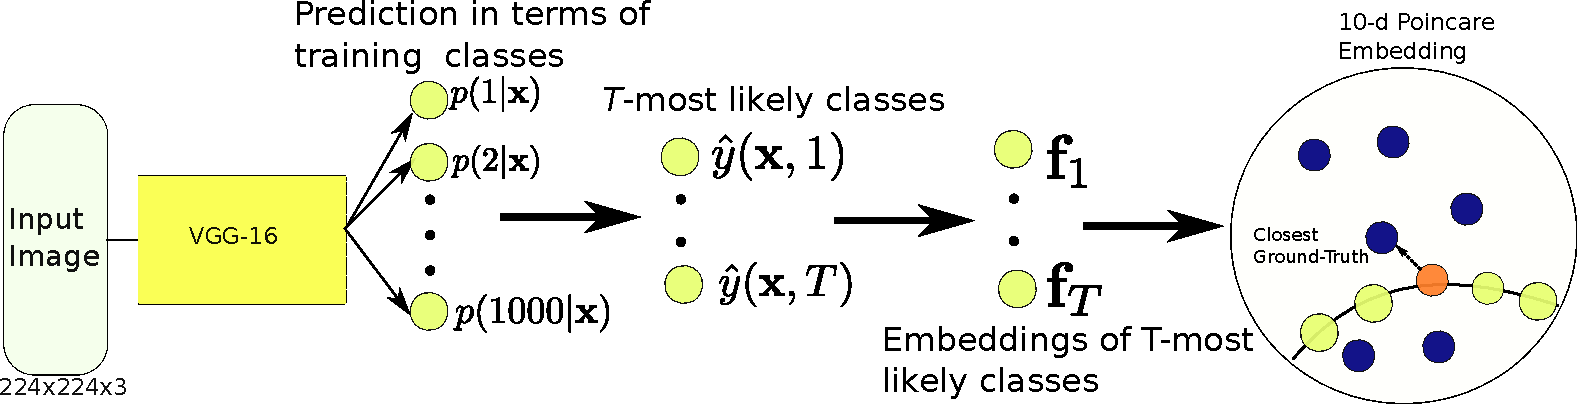
\includegraphics[width=\textwidth]{chsem}
  \caption{Illustration of the Convex-HSEM model. The orange circle represents the einstein midpoint of the semantic embeddings (yellow circles) of the $T$ most likely classes. The einstein midoint is mapped to the nearest ground-truth embedding in order to classify the input image}
  \label{fig:chsem}
\end{figure}

Since we used the pre-trained VGG-16 model, Convex-HSEM did not require any additional training and was therefore much faster to implement than the Deep-HSEM. The only hyperparameter to set was the number of data points over which to calculate the convex combination, $T$. We ran our experiments for 
$T \in \{1, 2, 5, 10, 100, 1000\}$. The motivation for this model architecture is to represent any unknown image as combination of known image classes. This model is hence predominantly aimed at zero-shot learning; if we were to classify a new image, and we knew it to be one of the 1000 training classes, it would make more sense just to use the standard VGG-16 model.

\newpage
\chapter{Conclusions \& Ideas for Future Work}

\section{Summary}
The aim of this thesis has been to improve the generalization ability of deep learning models used for image classification, and zero-shot learning in particular. The precise research question we set out to explore was: 
\begin{itemize}
\item \textit{Does semantic hierarchical knowledge in the form of hyperbolic embeddings help to improve the zero-shot prediction capability of deep learning models}
\end{itemize}
Two zero-shot learning models were introduced to investigate this: the Deep-Hyperbolic Semantic Embedding model used a CNN to learn a mapping from training images into a Poincare embedding, whilst the Convex-Hyperbolic Semantic Embedding model constructed embedding predictions as a weighted convex combination of known classes' embedding. Various zero-shot experiments were run on up to 21k previously unseen classes in an attempt to answer the above reserch question.

Overall our results show promising results \dots..versus Euclidean similarity based embeddings...The main contribution is therefore \dots.. However, as the next two sections highlight, there are several improvements that can be made in future works to explore this approach in more detail.

Whilst our hypebolic models did perform better on the robust zero-shot task, thus indicating the power of these models in learning hierarchical relations, their accuracy in non-zero shot and the standard zero-shot setting was worse. This suggests that \dots 

\section{Limitations \& Future Work}


a potential problem is dimensionality is it too low? especially we wish some local smoothness in therms of visual samples in embedding space.perhaps more dimensions are needed for this. Though hard to really say since hyperbolic space..

maybe different loss function; mse, distortion of xentropy, adding allemb to xentropy

need better embedding maybe lorenz, maybe higher dimensional and also maybe need ot learn mapping with not-just leaf nodes. In fact, if there is imprecision more at the leaf nodes, then by leanrig a mapping on them we may overfit. This maybe also why softmax works better than distanc

random poincare embeddings.
issues of training time
generalize zsl excluded.
more dimensions of the embedding space
new data sets e.g. if trained against embedding learns well new data sets
w2v model trained to same accuracy as poincare  

compare against state of the art -- we now havent, but would be interesting to see if their performance could be improved by Poincare embedding.
Numerical issues, attempted to use double-precision (64 bit floating points, more careful exploration of hyperparameters.












Big problem is that in the non-zero shot training the embedding model did much worse.

The main potential shortcomings of our model can be grouped under two broader, related, categories. The first ones have to do with the quality and usefulness of the hyperbolic semantic embedding built on the WordNet hierarchy, and the second ones have to with the quality of mapping we have learned from the image space into the embedding space.

Concerning the first set of limitations, it is clear from our analysis that there are certain situations in which our model performed worse than the baseline model that used similarity based worde embedding. One of the examples given was that of the word 'benthos' defined as 'organisms living at near the seabed'. Our model failed to classify this as it was not directly linked any species in the WordNet hierarchy. The baseline model had more success, persumably because the massive Wikipedia data used to create its embedding space had many species in the same context with 'benthos'. This illustrates that hierarchical semantic taxonomy is not alway better descriptor of visually relatedness than semantic contex. To be clear, this is not a shortcoming of hyperbolic embeddings in general, but rather a limitation of the WordNet versus the massive contextual data available from other data sets, in certain situations. In fact, future work could attempt to build a hyperbolic embedding based on both contextual data as well as explicit semantic word taxonomies. This is possible because the Poincare model of Nickel and Kiela \cite{Nickel2018} do not require excplicit hierarchy as an input, instead it just needs to be given data about which words are connected to each other. If such data set could be constructed from the Wikipedia data set, then we could use it to learn a latent hierarchy of those words and use that in conjunction with the Poincare embedding of this paper for improved performance. Another simpler approach may be to take a similarity based embedding model and our hyperbolic embedding model and always pick the most likely prediction across the two. 

The above issue is closely linked to the broader of problem of an embedding space not preserving the local structure of its input image space. This is a common challenge in zero-shot learning \cite{Ji2017}. Even if we didnt suffer from any of the potential problems discussed in the previous paragraph, it may be that no word-based semantic embedding can preserve visual structure smoothly. One possible way of dealing with this might be to use an approach similar to Kodirov \textit{et al.} \cite{Kodirov2017} in which the semantic embedding corresponds to the latent represenation layer of the autoencoder. We could improve on this by initializing the latent vectors to be those of the hyperbolic embedding, but make the vectors trainable. The reconstruction constraint of the autoencoder could thus help the model to re-adjust the initial hyperbolic embedding to be more visually smooth.
in combination with a hyperbolic embedding. 

Another common issue encountered in zero-shot learning is that of the domain projection shift \cite{Fu2015}; the training and test classes in zero-shot learning are fully disjoint and thus the learnt mapping may not transfer well. We suspect that this issue might be very relevant for hyperbolic embeddings on the ImageNet data. This is because a vast majority of the training labels are leaf nodes in the WordNet hierarchy and subsequently their locations in the hyperbolic embedding will be near to the border of the open unit ball. We hence effectively learning a mapping to only a constrained area of the hyperbolic space. This is likely exacerbated by the fact that almost 10\% \cite{Peterson2018} of the training image are specific dog breeds. A natural way future research could attempt to resolve this is by creating pseudo-exemplars for higher level visual categories. For instance, all the different images of 'mammals' could be clustered to find the sub-space of image features from where to sample these exemplars, which then could be used in training.

Finally, it would be worth exploring the possibility of imposing hyperbolic geometry on our model more broadly. For instance, Gulcehere \textit{et al.}, showed that placing hyperbolic geometry on the activation functions of neural networks can increase their representational capacity and improve performance. Currently only our embedding is in hyperbolic space and in training Riemannian gradients from the Poincare distance loss function are combined with Euclidean gradinets. If hyperbolic space was imposed on all model parameters, all the layers could be trained with Riemannian optimization. A more ambitous future research project would thus look at how this might be implemented and investigate its benefits on zero-shot learning.



\subsubsection{add}

On the otherhand, our ConSE model failed but this may be because Einstein midpoint is not great..

Possible issue runnign only 90 epochs

\bibliographystyle{ieeetr}
\bibliography{Thesis}

\end{document}
